\documentclass[a4paper,12pt]{article}

\usepackage[utf8]{inputenc}
\usepackage[english]{babel}
\usepackage{hyperref}
\usepackage{fontenc}
\usepackage{graphicx}
\usepackage{makeidx}
\usepackage{color}
\usepackage{multirow}
\usepackage{tabularx}
\usepackage{longtable}
\usepackage{url}
\usepackage{titlesec}
\usepackage{listings}
\usepackage{xcolor}
\usepackage{colortbl}
\usepackage{geometry}
\usepackage{pdflscape}

\geometry{
    a4paper,
    left=25mm,
    right=25mm,
    top=30mm,
    bottom=30mm,
 }

%%%%%%%%%%%%%%%%%%%%%%%%%%%%%
%%%%%%% CONFIGURATION %%%%%%%
%%%%%%%%%%%%%%%%%%%%%%%%%%%%%
%%%%%%%%%%%%%%%%%%%%%%%%%%%%%%%%%%%%%%
%%%%%%% SECTION CONFIGURATIONS %%%%%%%
%%%%%%%%%%%%%%%%%%%%%%%%%%%%%%%%%%%%%%
\newcommand{\sectionbreak}{\clearpage}

\setcounter{secnumdepth}{5}

\titleformat{\paragraph}
{\normalfont\normalsize\bfseries}{\theparagraph}{1em}{}
\titlespacing*{\paragraph}
{0pt}{3.25ex plus 1ex minus .2ex}{1.5ex plus .2ex}


%%%%%%%%%%%%%%%%%%%%%%%%%%%%%%%%%%%%%%
%%%%%%% LISTINGS CONFIGURATION %%%%%%%
%%%%%%%%%%%%%%%%%%%%%%%%%%%%%%%%%%%%%%
\definecolor{mybg}{rgb}{1,1,0.8}
\definecolor{mysoftblue}{rgb}{0.6,0.729,0.867}
\definecolor{mygreen}{rgb}{0,0.6,0}
\definecolor{mygray}{rgb}{0.5,0.5,0.5}
\definecolor{mymauve}{rgb}{0.58,0,0.82}

\lstset{ %
  backgroundcolor=\color{mysoftblue},    % choose the background color; you must add \usepackage{color} or \usepackage{xcolor}
  basicstyle=\ttfamily\scriptsize,        % the size of the fonts that are used for the code
  breakatwhitespace=false,         % sets if automatic breaks should only happen at whitespace
  breaklines=true,                 % sets automatic line breaking
  captionpos=b,                    % sets the caption-position to bottom
  commentstyle=\color{mygreen},    % comment style
  deletekeywords={...},            % if you want to delete keywords from the given language
  escapeinside={\%*}{*)},          % if you want to add LaTeX within your code (example: \%* int v; *) )
  extendedchars=true,              % lets you use non-ASCII characters; for 8-bits encodings only, does not work with UTF-8
  frame=single,                    % adds a frame around the code (none, single)
  keepspaces=true,                 % keeps spaces in text, useful for keeping indentation of code (possibly needs columns=flexible)
  keywordstyle=\color{blue},       % keyword style
  language=Java,                   % the language of the code
  otherkeywords={*,...},           % if you want to add more keywords to the set
  numbers=none,                    % where to put the line-numbers; possible values are (none, left, right)
  numbersep=5pt,                   % how far the line-numbers are from the code
  numberstyle=\tiny\color{mygray}, % the style that is used for the line-numbers
  rulecolor=\color{black},         % if not set, the frame-color may be changed on line-breaks within not-black text (e.g. comments (green here))
  showspaces=false,                % show spaces everywhere adding particular underscores; it overrides 'showstringspaces'
  showstringspaces=false,          % underline spaces within strings only
  showtabs=false,                  % show tabs within strings adding particular underscores
  stepnumber=2,                    % the step between two line-numbers. If it's 1, each line will be numbered
  stringstyle=\color{mymauve},     % string literal style
  tabsize=2,                       % sets default tabsize to 2 spaces
  title=\lstname,                  % show the filename of files included with \lstinputlisting; also try caption instead of title
  aboveskip=20pt,                  % space left avobe the listing
  belowskip=0pt,                   % space left below the listing
  columns=fullflexible             % to allow automatic copy from listings
}


%%%%%%%%%%%%%%%%%%%%%%%%%%%%%%%%%%%
%%%%%%% OTHER CONFIGURATION %%%%%%%
%%%%%%%%%%%%%%%%%%%%%%%%%%%%%%%%%%%

% Horizontal line
\newcommand{\HRule}{
  \rule{\linewidth}{0.5mm}
}

% Color box for comments
\newcommand{\colorComment}[1]{
\begin{table}[h]
    \centering
    \begin{tabular}{p{0.8\textwidth}}
        \cellcolor{orange}\begin{center}
	  #1 \\
        \end{center}
        \\
    \end{tabular}
\end{table}
}
\title{COMP Superscalar}
\author{User Guide: Application development guide}
\def \compssversion {2.5.rc1906}

\makeindex

%%%%%%%%%%%%%%%%%%%%%%%%%%%%%
%%%%%%%% DOCUMENT %%%%%%%%%%%
%%%%%%%%%%%%%%%%%%%%%%%%%%%%%
\begin{document}

  %%%%%%%%%%%% TITLE PAGE %%%%%%%%%%%%%
  \hypersetup{pageanchor=false}
  \begin{titlepage} 
    \begin{center} 
      
\includegraphics[width=0.3\textwidth]{./Figures/Logos/degradado-naranja-compss.jpg}~\\[1cm] 
      \textsc{\LARGE COMP Superscalar}\\[1.5cm] 
      
      \HRule \\[0.4cm] 
      { \huge \bfseries User Manual \\[0.4cm] }
      { \large \bfseries Application development guide \\[0.4cm] } 
      \HRule \\[1.5cm] 

      { \large \textsc{Version: \compssversion}} \\[0.3cm]
      { \large \today }

      \vfill 
      % Bottom of the page
      
\includegraphics[width=0.5\textwidth]{./Figures/bsc_280.jpg}~\\[1cm]
    \end{center} 
  \end{titlepage}
  \hypersetup{pageanchor=true}
  
  %%%%%%%% REFERENCE NOTES %%%%%%%%%%
  {
    This manual only provides information about the development of COMPSs applications. Specifically, it details
    the programming model features available in Java, Python and C/C++ languages. 
    \newline
    
    For an extensive list of COMPSs application examples (codes, execution commands, results, logs, etc.) please refer to the \textit{COMPSs Sample 
    Applications} guide at \url{http://compss.bsc.es/} .
    \newline
    
    For information about the installation process please refer to the \textit{COMPSs Installation Guide} available at
    \url{http://compss.bsc.es/} .
    \newline
    
    For further information about the application execution please refer to the \textit{COMPSs User Manual: Application execution 
    guide} available at \url{http://compss.bsc.es/} .
    \newline
  }
  
  %%%%%%%% TABLE OF CONTENTS %%%%%%%%%%
  \pagenumbering{roman}
  \setcounter{tocdepth}{6}
  \tableofcontents
  \listoffigures
  \listoftables
    
  \newpage

  %%%%%%%%%%%%% CONTENTS %%%%%%%%%%%%%%
  \pagenumbering{arabic}
    
  \section{COMP Superscalar (COMPSs)}
\label{sec:Introduction}

COMP Superscalar (COMPSs) is a programming model which aims to ease the development of applications for distributed infrastructures, such as Clusters, Grids and Clouds. COMP superscalar also features a runtime system that exploits the inherent parallelism of applications at execution time.

For the sake of programming productivity, the COMPSs model has four key characteristics:

\begin{itemize}
 
 \item  {\bf Sequential programming:} COMPSs programmers do not need to deal with the typical duties of parallelization and distribution, such as thread creation and synchronization, data distribution, messaging or fault tolerance. Instead, the model is based on sequential programming, which makes it appealing to users that either lack parallel programming expertise or are looking for better programmability.
 
 \item  {\bf Infrastructure unaware:} COMPSs offers a model that abstracts the application from the underlying distributed infrastructure. Hence, COMPSs programs do not include any detail that could tie them to a particular platform, like deployment or resource management. This makes applications portable between infrastructures with diverse characteristics.
 
 \item  {\bf Standard programming languages:} COMPSs is based on the popular programming language Java, but also offers language bindings for Python and C/C++ applications. This facilitates the learning of the model, since programmers can reuse most of their previous knowledge.
 
 \item  {\bf No APIs:} In the case of COMPSs applications in Java, the model does not require to use any special API call, pragma or construct in the application; everything is pure standard Java syntax and libraries. With regard the Python and C/C++ bindings, a small set of API calls should be used on the COMPSs applications.

\end{itemize}


  
  \section{Java Sample applications}
\label{sec:JavaSampleApps}

The first two examples in this section are simple applications developed in COMPSs to easily illustrate how to code,
compile and run COMPSs applications. These applications are executed locally and show different ways to take advantage
of all the COMPSs features. 

The rest of the examples are more elaborated and consider the execution in a cloud platform where the VMs mount a common 
storage on \textbf{/sharedDisk} directory. This is useful in the case of applications that require working 
with big files, allowing to transfer data only once, at the beginning of the execution, and to enable 
the application to access the data directly during the rest of the execution.

The Virtual Machine available at our webpage (\url{http://compss.bsc.es/}) provides a development environment with
all the applications listed in the following sections. The codes of all the applications can be found under the 
$/home/compss/tutorial\_apps/java/$ folder. 

%%%%%%%%%%%%%%%
%% HELLO WORLD 
%%%%%%%%%%%%%%%
\subsection{Hello World}
The Hello Wolrd is a Java application that creates a task and prints a Hello World! message. Its purpose is to clarify that the 
COMPSs tasks output is redirected to the job files and it is \textbf{not} available at the standard output. 

Next we provide the important parts of the application's code.

\begin{lstlisting}[language=java]
	// hello.Hello
	
	public static void main(String[] args) throws Exception {
		// Check and get parameters
		if (args.length != 0) {
			usage();
			throw new Exception("[ERROR] Incorrect number of parameters");
		}
		
		// Hello World from main application
		System.out.println("Hello World! (from main application)");

		// Hello World from a task
		HelloImpl.sayHello();
	}
\end{lstlisting}

As shown in the main code, this application has no input arguments. 

\begin{lstlisting}[language=java]
	// hello.HelloImpl
	
	public static void sayHello() {
		System.out.println("Hello World! (from a task)");
	}
\end{lstlisting}

Remember that, to run with COMPSs, java applications must provide an interface. For simplicity, in this example, the content of the interface only
declares the task which has no parameters:

\begin{lstlisting}[language=java]
	// hello.HelloItf
	
	@Method(declaringClass = "hello.HelloImpl")
	void sayHello(
	);
\end{lstlisting}

Notice that there is a first Hello World message printed from the main code and, a second one, printed inside a task. When executing sequentially
this application users will be able to see both messages at the standard output. However, when executing this application with COMPSs, users will only
see the message from the main code at the standard output. The message printed from the task will be stored inside the job log files. 

Let's try it. First we proceed to compile the code by running the following instructions:

\begin{lstlisting}[language=bash]
compss@bsc:~$ cd ~/tutorial_apps/java/hello/src/main/java/hello/
compss@bsc:~/tutorial_apps/java/hello/src/main/java/hello$ javac *.java
compss@bsc:~/tutorial_apps/java/hello/src/main/java/hello$ cd ..
compss@bsc:~/tutorial_apps/java/hello/src/main/java$ jar cf hello.jar hello
compss@bsc:~/tutorial_apps/java/hello/src/main/java$ mv hello.jar ~/tutorial_apps/java/hello/jar/
\end{lstlisting}

Alternatively, this example application is prepared to be compiled with \textit{maven}:

\begin{lstlisting}[language=bash]
compss@bsc:~$ cd ~/tutorial_apps/java/hello/
compss@bsc:~/tutorial_apps/java/hello$ mvn clean package
\end{lstlisting}

Once done, we can sequentially execute the application by directly invoking the \textit{jar} file.

\begin{lstlisting}[language=bash]
compss@bsc:~$ cd ~/tutorial_apps/java/hello/jar/
compss@bsc:~/tutorial_apps/java/hello/jar$ java -cp hello.jar hello.Hello 
Hello World! (from main application)
Hello World! (from a task)
\end{lstlisting}

And we can also execute the application with COMPSs:

\begin{lstlisting}[language=bash]
compss@bsc:~$ cd ~/tutorial_apps/java/hello/jar/
compss@bsc:~/tutorial_apps/java/hello/jar$ runcompss -d hello.Hello
[  INFO] Using default execution type: compss
[  INFO] Using default location for project file: /opt/COMPSs/Runtime/configuration/xml/projects/default_project.xml
[  INFO] Using default location for resources file: /opt/COMPSs/Runtime/configuration/xml/resources/default_resources.xml

----------------- Executing hello.Hello --------------------------

WARNING: IT Properties file is null. Setting default values
[(928)    API]  -  Deploying COMPSs Runtime v<version>
[(931)    API]  -  Starting COMPSs Runtime v<version>
[(931)    API]  -  Initializing components
[(1472)    API]  -  Ready to process tasks
Hello World! (from main application)
[(1474)    API]  -  Creating task from method sayHello in hello.HelloImpl
[(1474)    API]  -  There is 0 parameter
[(1477)    API]  -  No more tasks for app 1
[(4029)    API]  -  Getting Result Files 1
[(4030)    API]  -  Stop IT reached
[(4030)    API]  -  Stopping AP...
[(4031)    API]  -  Stopping TD...
[(4161)    API]  -  Stopping Comm...
[(4163)    API]  -  Runtime stopped
[(4166)    API]  -  Execution Finished

------------------------------------------------------------
\end{lstlisting}

Notice that the COMPSs execution is using the \textit{-d} option to allow the job logging. Thus, we can check out the application jobs folder to look for
the task output.

\begin{lstlisting}[language=bash]
compss@bsc:~$ cd ~/.COMPSs/hello.Hello_01/jobs/
compss@bsc:~/.COMPSs/hello.Hello_01/jobs$ ls -1
job1_NEW.err
job1_NEW.out
compss@bsc:~/.COMPSs/hello.Hello_01/jobs$ cat job1_NEW.out
[JAVA EXECUTOR] executeTask - Begin task execution
WORKER - Parameters of execution:
  * Method type: METHOD
  * Method definition: [DECLARING CLASS=hello.HelloImpl, METHOD NAME=sayHello]
  * Parameter types:
  * Parameter values:
Hello World! (from a task)
[JAVA EXECUTOR] executeTask - End task execution
\end{lstlisting}

%%%%%%%%%%%%%%%
%% SIMPLE
%%%%%%%%%%%%%%%
\subsection{Simple}
The Simple application is a Java application that increases a counter by means of a task. The counter is stored inside a file that 
is transferred to the worker when the task is executed. Thus, the tasks inferface is defined as follows:

\begin{lstlisting}[language=java]
	// simple.SimpleItf
	
	@Method(declaringClass = "simple.SimpleImpl")
	void increment(
		@Parameter(type = Type.FILE, direction = Direction.INOUT) String file
	);
\end{lstlisting}

Next we also provide the invocation of the task from the main code and the increment's method code.

\begin{lstlisting}[language=java]
	// simple.Simple
	
	public static void main(String[] args) throws Exception {
		// Check and get parameters
		if (args.length != 1) {
			usage();
			throw new Exception("[ERROR] Incorrect number of parameters");
		}
		int initialValue = Integer.parseInt(args[0]);

		// Write value
		FileOutputStream fos = new FileOutputStream(fileName);
		fos.write(initialValue);
		fos.close();
		System.out.println("Initial counter value is " + initialValue);

		//Execute increment
		SimpleImpl.increment(fileName);

		// Write new value
		FileInputStream fis = new FileInputStream(fileName);
		int finalValue = fis.read();
		fis.close();
		System.out.println("Final counter value is " + finalValue);
	}
\end{lstlisting}

\begin{lstlisting}[language=java]
	// simple.SimpleImpl
	
	public static void increment(String counterFile) throws FileNotFoundException, IOException {
		// Read value
		FileInputStream fis = new FileInputStream(counterFile);
		int count = fis.read();
		fis.close();
		
		// Write new value
		FileOutputStream fos = new FileOutputStream(counterFile);
		fos.write(++count);
		fos.close();
	}
\end{lstlisting}

Finally, to compile and execute this application users must run the following commands:

\begin{lstlisting}[language=bash]
compss@bsc:~$ cd ~/tutorial_apps/java/simple/src/main/java/simple/
compss@bsc:~/tutorial_apps/java/simple/src/main/java/simple$ javac *.java
compss@bsc:~/tutorial_apps/java/simple/src/main/java/simple$ cd ..
compss@bsc:~/tutorial_apps/java/simple/src/main/java$ jar cf simple.jar simple
compss@bsc:~/tutorial_apps/java/simple/src/main/java$ mv simple.jar ~/tutorial_apps/java/simple/jar/

compss@bsc:~$ cd ~/tutorial_apps/java/simple/jar
compss@bsc:~/tutorial_apps/java/simple/jar$ runcompss simple.Simple 1
compss@bsc:~/tutorial_apps/java/simple/jar$ runcompss simple.Simple 1
[  INFO] Using default execution type: compss
[  INFO] Using default location for project file: /opt/COMPSs/Runtime/configuration/xml/projects/default_project.xml
[  INFO] Using default location for resources file: /opt/COMPSs/Runtime/configuration/xml/resources/default_resources.xml

----------------- Executing simple.Simple --------------------------

WARNING: IT Properties file is null. Setting default values
[(772)    API]  -  Starting COMPSs Runtime v<version>
Initial counter value is 1
Final counter value is 2
[(3813)    API]  -  Execution Finished

------------------------------------------------------------
\end{lstlisting}


%%%%%%%%%%%%%%%
%% Increment
%%%%%%%%%%%%%%%
\subsection{Increment}
The Increment application is a Java application that increases N times three different counters. Each increase step is developed by a separated task. The
purpose of this application is to show parallelism between the three counters.

Next we provide the main code of this application. The code inside the \textit{increment} task is the same than the previous example. 

\begin{lstlisting}[language=java]
	// increment.Increment
	public static void main(String[] args) throws Exception {
		// Check and get parameters
		if (args.length != 4) {
			usage();
			throw new Exception("[ERROR] Incorrect number of parameters");
		}
		int N = Integer.parseInt(args[0]);
		int counter1 = Integer.parseInt(args[1]);
		int counter2 = Integer.parseInt(args[2]);
		int counter3 = Integer.parseInt(args[3]);
		
		// Initialize counter files
		System.out.println("Initial counter values:");
		initializeCounters(counter1, counter2, counter3);
		
		// Print initial counters state
		printCounterValues();

		// Execute increment tasks
		for (int i = 0; i < N; ++i) {
			IncrementImpl.increment(fileName1);
			IncrementImpl.increment(fileName2);
			IncrementImpl.increment(fileName3);
		}

		// Print final counters state (sync)
		System.out.println("Final counter values:");
		printCounterValues();
	}
\end{lstlisting}

As shown in the main code, this application has 4 parameters that stand for:

\begin{enumerate}
 \item \textbf{N:} Number of times to increase a counter
 \item \textbf{InitialValue1:} Initial value for counter 1
 \item \textbf{InitialValue2:} Initial value for counter 2
 \item \textbf{InitialValue3:} Initial value for counter 3
\end{enumerate}

Next we will compile and run the Increment application with the \textit{-g} option to be able to generate the final graph at the end of the execution.

\begin{lstlisting}[language=bash]
compss@bsc:~$ cd ~/tutorial_apps/java/increment/src/main/java/increment/
compss@bsc:~/tutorial_apps/java/increment/src/main/java/increment$ javac *.java
compss@bsc:~/tutorial_apps/java/increment/src/main/java/increment$ cd ..
compss@bsc:~/tutorial_apps/java/increment/src/main/java$ jar cf increment.jar increment
compss@bsc:~/tutorial_apps/java/increment/src/main/java$ mv increment.jar ~/tutorial_apps/java/increment/jar/

compss@bsc:~$ cd ~/tutorial_apps/java/increment/jar
compss@bsc:~/tutorial_apps/java/increment/jar$ runcompss -g increment.Increment 10 1 2 3
[  INFO] Using default execution type: compss
[  INFO] Using default location for project file: /opt/COMPSs/Runtime/configuration/xml/projects/default_project.xml
[  INFO] Using default location for resources file: /opt/COMPSs/Runtime/configuration/xml/resources/default_resources.xml

----------------- Executing increment.Increment --------------------------

WARNING: IT Properties file is null. Setting default values
[(1028)    API]  -  Starting COMPSs Runtime v<version>
Initial counter values:
- Counter1 value is 1
- Counter2 value is 2
- Counter3 value is 3
Final counter values:
- Counter1 value is 11
- Counter2 value is 12
- Counter3 value is 13
[(4403)    API]  -  Execution Finished

------------------------------------------------------------
\end{lstlisting}

By running the \textit{gengraph} command users can obtain the task graph of the above execution. Next we provide the set of commands to obtain the
graph show in Figure \ref{fig:increment_java}.

\begin{lstlisting}[language=bash]
compss@bsc:~$ cd ~/.COMPSs/increment.Increment_01/monitor/
compss@bsc:~/.COMPSs/increment.Increment_01/monitor$ gengraph complete_graph.dot
compss@bsc:~/.COMPSs/increment.Increment_01/monitor$ evince complete_graph.pdf
\end{lstlisting}

\begin{figure}[ht!]
  \centering
    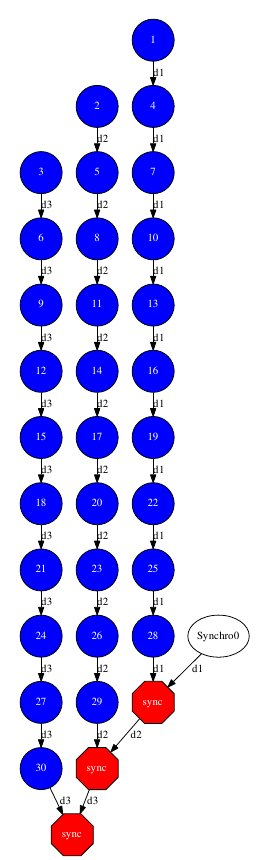
\includegraphics[width=0.3\textwidth]{./Sections/2_Java/Figures/increment_graph.jpeg}
    \caption{Java increment tasks graph} 
    \label{fig:increment_java}
\end{figure}

%%%%%%%%%%%%%%%
%% MATMUL
%%%%%%%%%%%%%%%
\newpage
\subsection{Matrix multiplication}
The Matrix Multiplication (Matmul) is a pure Java application that multiplies two matrices in a direct way. 
The application creates 2 matrices of N x N size initialized with values, and multiply the matrices by blocks.

This application provides three different implementations that only differ on the way of storing the matrix:
\begin{enumerate}
 \item \textbf{matmul.objects.Matmul} Matrix stored by means of objects
 \item \textbf{matmul.files.Matmul} Matrix stored in files
 \item \textbf{matmul.arrays.Matmul} Matrix represented by an array
\end{enumerate}

\begin{figure}[ht!]
  \centering
    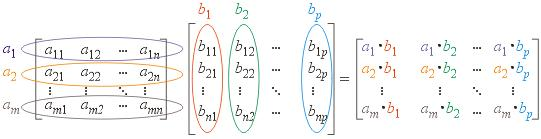
\includegraphics[width=0.8\textwidth]{./Sections/2_Java/Figures/matrix.jpeg}
    \caption{Matrix multiplication} 
    \label{fig:matrix}
\end{figure}

\newpage 
In all the implementations the multiplication is implemented in the multiplyAccumulative method that is thus selected as the task to be executed remotely.
As example, we we provide next the task implementation and the tasks interface for the objects implementation.

\begin{lstlisting}[language=java]
	// matmul.objects.Block
	public void multiplyAccumulative(Block a, Block b) {
		for (int i = 0; i < M; i++) {
			for (int j = 0; j < M; j++) {
				for (int k = 0; k < M; k++) {
					data[i][j] += a.data[i][k]*b.data[k][j];
				}
			}
		}
	}
\end{lstlisting}

\begin{lstlisting}[language=java]
	// matmul.objects.MatmulItf
	@Method(declaringClass = "matmul.objects.Block")
	void multiplyAccumulative(
		@Parameter Block a,
		@Parameter Block b
	);
\end{lstlisting}

In order to run the application the matrix dimension (number of blocks) and the dimension of each block have to be supplied. Consequently, any of the 
implementations must be executed by running the following command.
\begin{lstlisting}[language=bash]
compss@bsc:~$ runcompss matmul.<IMPLEMENTATION_TYPE>.Matmul <matrix_dim> <block_dim>
\end{lstlisting}

Finally, we provide an example of execution for each implementation.

\begin{lstlisting}[language=bash]
compss@bsc:~$ cd ~/tutorial_apps/java/matmul/jar/
compss@bsc:~/tutorial_apps/java/matmul/jar$ runcompss matmul.objects.Matmul 8 4
[  INFO] Using default execution type: compss
[  INFO] Using default location for project file: /opt/COMPSs/Runtime/configuration/xml/projects/default_project.xml
[  INFO] Using default location for resources file: /opt/COMPSs/Runtime/configuration/xml/resources/default_resources.xml

----------------- Executing matmul.objects.Matmul --------------------------

WARNING: IT Properties file is null. Setting default values
[(887)    API]  -  Starting COMPSs Runtime v<version>
[LOG] MSIZE parameter value = 8
[LOG] BSIZE parameter value = 4
[LOG] Allocating A/B/C matrix space
[LOG] Computing Result
[LOG] Main program finished.
[(7415)    API]  -  Execution Finished

------------------------------------------------------------
\end{lstlisting}

\begin{lstlisting}[language=bash]
compss@bsc:~$ cd ~/tutorial_apps/java/matmul/jar/
compss@bsc:~/tutorial_apps/java/matmul/jar$ runcompss matmul.files.Matmul 8 4
[  INFO] Using default execution type: compss
[  INFO] Using default location for project file: /opt/COMPSs/Runtime/configuration/xml/projects/default_project.xml
[  INFO] Using default location for resources file: /opt/COMPSs/Runtime/configuration/xml/resources/default_resources.xml

----------------- Executing matmul.files.Matmul --------------------------

WARNING: IT Properties file is null. Setting default values
[(907)    API]  -  Starting COMPSs Runtime v<version>
[LOG] MSIZE parameter value = 8
[LOG] BSIZE parameter value = 4
[LOG] Computing result
[LOG] Main program finished.
[(9925)    API]  -  Execution Finished

------------------------------------------------------------
\end{lstlisting}


\begin{lstlisting}[language=bash]
compss@bsc:~$ cd ~/tutorial_apps/java/matmul/jar/
compss@bsc:~/tutorial_apps/java/matmul/jar$ runcompss matmul.arrays.Matmul 8 4
[  INFO] Using default execution type: compss
[  INFO] Using default location for project file: /opt/COMPSs/Runtime/configuration/xml/projects/default_project.xml
[  INFO] Using default location for resources file: /opt/COMPSs/Runtime/configuration/xml/resources/default_resources.xml

----------------- Executing matmul.arrays.Matmul --------------------------

WARNING: IT Properties file is null. Setting default values
[(1062)    API]  -  Starting COMPSs Runtime v<version>
[LOG] MSIZE parameter value = 8
[LOG] BSIZE parameter value = 4
[LOG] Allocating C matrix space
[LOG] Computing Result
[LOG] Main program finished.
[(7811)    API]  -  Execution Finished

------------------------------------------------------------
\end{lstlisting}


%%%%%%%%%%%%%%%
%% SPARSELU 
%%%%%%%%%%%%%%%
\subsection{Sparse LU decomposition}
SparseLU multiplies two matrices using the factorization method of LU decomposition, which factorizes a 
matrix as a product of a lower triangular matrix and an upper one.

\begin{figure}[ht!]
  \centering
    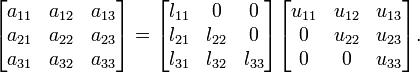
\includegraphics[width=0.6\textwidth]{./Sections/2_Java/Figures/SparseLU.jpeg}
    \caption{Sparse LU decomposition}
    \label{fig:SparseLO}
\end{figure}

The matrix is divided into N x N blocks on where 4 types of operations will be applied modifying the blocks: 
{\bf lu0}, {\bf fwd}, {\bf bdiv} and {\bf bmod}. These four operations are implemented in four methods that 
are selecetd as the tasks that will be executed remotely. In order to run the application the matrix dimension 
has to be provided.

As the previous application, the sparseLU is provided in three different implementations that only differ on the way of storing
the matrix:
\begin{enumerate}
 \item \textbf{sparseLU.objects.SparseLU} Matrix stored by means of objects
 \item \textbf{sparseLU.files.SparseLU} Matrix stored in files
 \item \textbf{sparseLU.arrays.SparseLU} Matrix represented by an array
\end{enumerate}

Thus, the commands needed to execute the application is with each implementation are:

\begin{lstlisting}[language=bash]
compss@bsc:~$ cd tutorial_apps/java/sparseLU/jar/
compss@bsc:~/tutorial_apps/java/sparseLU/jar$ runcompss sparseLU.objects.SparseLU 16 8
[  INFO] Using default execution type: compss
[  INFO] Using default location for project file: /opt/COMPSs/Runtime/configuration/xml/projects/default_project.xml
[  INFO] Using default location for resources file: /opt/COMPSs/Runtime/configuration/xml/resources/default_resources.xml

----------------- Executing sparseLU.objects.SparseLU --------------------------

WARNING: IT Properties file is null. Setting default values
[(1221)    API]  -  Starting COMPSs Runtime v<version>
[LOG] Running with the following parameters:
[LOG]  - Matrix Size: 16
[LOG]  - Block Size:  8
[LOG] Initializing Matrix
[LOG] Computing SparseLU algorithm on A
[LOG] Main program finished.
[(13642)    API]  -  Execution Finished

------------------------------------------------------------
\end{lstlisting}

\begin{lstlisting}[language=bash]
compss@bsc:~$ cd tutorial_apps/java/sparseLU/jar/
compss@bsc:~/tutorial_apps/java/sparseLU/jar$ runcompss sparseLU.files.SparseLU 4 8
[  INFO] Using default execution type: compss
[  INFO] Using default location for project file: /opt/COMPSs/Runtime/configuration/xml/projects/default_project.xml
[  INFO] Using default location for resources file: /opt/COMPSs/Runtime/configuration/xml/resources/default_resources.xml

----------------- Executing sparseLU.files.SparseLU --------------------------

WARNING: IT Properties file is null. Setting default values
[(1082)    API]  -  Starting COMPSs Runtime v<version>
[LOG] Running with the following parameters:
[LOG]  - Matrix Size: 16
[LOG]  - Block Size:  8
[LOG] Initializing Matrix
[LOG] Computing SparseLU algorithm on A
[LOG] Main program finished.
[(13605)    API]  -  Execution Finished

------------------------------------------------------------

\end{lstlisting}

\begin{lstlisting}[language=bash]
compss@bsc:~$ cd tutorial_apps/java/sparseLU/jar/
compss@bsc:~/tutorial_apps/java/sparseLU/jar$ runcompss sparseLU.arrays.SparseLU 8 8
[  INFO] Using default execution type: compss
[  INFO] Using default location for project file: /opt/COMPSs/Runtime/configuration/xml/projects/default_project.xml
[  INFO] Using default location for resources file: /opt/COMPSs/Runtime/configuration/xml/resources/default_resources.xml

----------------- Executing sparseLU.arrays.SparseLU --------------------------

WARNING: IT Properties file is null. Setting default values
[(1082)    API]  -  Starting COMPSs Runtime v<version>
[LOG] Running with the following parameters:
[LOG]  - Matrix Size: 16
[LOG]  - Block Size:  8
[LOG] Initializing Matrix
[LOG] Computing SparseLU algorithm on A
[LOG] Main program finished.
[(13605)    API]  -  Execution Finished

------------------------------------------------------------

\end{lstlisting}


%%%%%%%%%%%%%%%
%% KMEANS
%%%%%%%%%%%%%%%
%\subsection{KMeans}


%%%%%%%%%%%%%%%
%% BLAST
%%%%%%%%%%%%%%%
\subsection{BLAST Workflow}
BLAST is a widely-used bioinformatics tool for comparing primary biological sequence information, such as 
the amino-acid sequences of different proteins or the nucleotides of DNA sequences with sequence databases, 
identifying sequences that resemble the query sequence above a certain threshold. 
The work performed by the COMPSs Blast workflow is computationally intensive and embarrassingly parallel.

\begin{figure}[ht!]
  \centering
    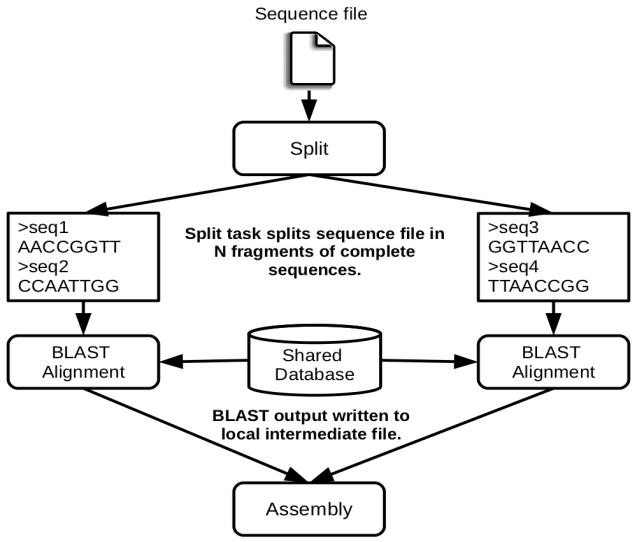
\includegraphics[width=0.7\textwidth]{./Sections/2_Java/Figures/blast_workflow.jpeg}
    \caption{The COMPSs Blast workflow}
    \label{fig:BLAST_workflow}
\end{figure}

The workflow describes the three blocks of the workflow implemented in the {\bf Split}, {\bf Align} and 
{\bf Assembly} methods. The second one is the only method that is chosen to be executed remotely, so it 
is the unique method defined in the interface file. The {\bf Split} method chops the query sequences file 
in N fragments, {\bf Align} compares each sequence fragment against the database by means of the Blast 
binary, and {\bf Assembly} combines all intermediate files into a single result file.

This application uses a database that will be on the shared disk space avoiding transferring the entire 
database (which can be large) between the virtual machines.

\begin{lstlisting}[language=bash]
compss@bsc:~$ cp ~/workspace/blast/package/Blast.tar.gz /home/compss/
compss@bsc:~$ tar xzf Blast.tar.gz
\end{lstlisting}

The command line to execute the workflow:

\begin{lstlisting}[language=bash]
compss@bsc:~$ runcompss blast.Blast <debug> 
                                    <bin_location>
                                    <database_file> 
                                    <sequences_file>
                                    <frag_number> 
                                    <tmpdir>
                                    <output_file>
\end{lstlisting}

Where:
\begin{itemize}
 \item {\bf debug}: The debug flag of the application (true or false).
 \item {\bf bin\_location}: Path of the Blast binary.
 \item {\bf database\_file}: Path of database file; the shared disk {\bf /sharedDisk/} is suggested to avoid big data transfers.
 \item {\bf sequences\_file}: Path of sequences file.
 \item {\bf frag\_number}: Number of fragments of the original sequence file, this number determines the number of parallel Align tasks.
 \item {\bf tmpdir}: Temporary directory ({\bf /home/compss/tmp/}).
 \item {\bf output\_file}: Path of the result file.
\end{itemize}
 
Example:
\begin{lstlisting}[language=bash]
compss@bsc:~$ runcompss blast.Blast true
                        /home/compss/tutorial_apps/java/blast/binary/blastall
                        /sharedDisk/Blast/databases/swissprot/swissprot
                        /sharedDisk/Blast/sequences/sargasso_test.fasta 
                        4 
                        /tmp/
                        /home/compss/out.txt
\end{lstlisting}
  
  \section{Python Binding}
\label{sec:Python}

COMPSs features a binding for Python 2 and 3 applications. 
The next subsections explain how to program a Python application for COMPSs and a brief overview on how to execute it.

\subsection{Programming Model}
\label{subsec:Python_programming_model}

\subsubsection{Task Selection}

As in the case of Java, a COMPSs Python application is a Python sequential program that contains calls to tasks. 
In particular, the user can select as a task:

\begin{itemize}
 \item Functions
 \item Instance methods: methods invoked on objects.
 \item Class methods: static methods belonging to a class.
\end{itemize}

The task definition in Python is done by means of Python decorators instead of an annotated interface. 
In particular, the user needs to add a {\it $@$task} decorator that describes the task before the definition of the function/method.

As an example, let us assume that the application calls a function \textit{func}, which receives a file path (string parameter) 
and an integer parameter. The code of \textit{func} updates the file.

\begin{lstlisting}[language=python]
def func(file_path, value):
    # update the file 'file_path'

if __name__=='__main__':
    my_file = '/tmp/sample_file.txt'
    func(my_file, 1)
\end{lstlisting}

Please, note that the main code is defined within \emph{if \_\_name\_\_==\'\_\_main\_\_\'}.
A better alternative would be to define the main code within a function and invoke it from the \emph{if \_\_name\_\_==\'\_\_main\_\_\'}.

In order to select {\it func} as a task, the corresponding {\it $@$task} decorator needs to be placed right 
before the definition of the function, providing some metadata about the parameters of that function. 
The {\it $@$task} decorator has to be imported from the {\it pycompss} library:

\begin{lstlisting}[language=python]
from pycompss.api.task import task
\end{lstlisting}

The metadata corresponding to a parameter is specified as an argument of the decorator, whose name is 
the formal parameter's name and whose value defines the type and direction of the parameter. 
The parameter types and directions can be:

\begin{itemize}
 \item Types: {\it primitive types} (integer, long, float, boolean), {\it strings}, {\it objects} (instances of user-defined classes, dictionaries, lists, tuples, complex numbers) and {\it files} are supported.
 \item Direction: it can be read-only ({\it IN} - default), read-write ({\it INOUT}), write-only ({\it OUT}) or in some cases concurrent ({\it CONCURRENT}).
\end{itemize}

COMPSs is able to automatically infer the parameter type for primitive types, strings and objects, 
while the user needs to specify it for files. On the other hand, the direction is only mandatory for 
{\it INOUT} and {\it OUT} parameters. Thus, when defining the parameter metadata in the {\it $@$task} 
decorator, the user has the following options:

\begin{itemize}
 \item {\it IN}: the parameter is read-only. The type will be inferred.
 \item {\it INOUT}: the parameter is read-write. The type will be inferred.
 \item {\it OUT}: the parameter is write-only. The type will be inferred.
 \item {\it CONCURRENT}: the parameter is read-write with concurrent acces. The type will be inferred.
 \item {\it FILE/FILE\_IN}: the parameter is a file. The direction is assumed to be {\it IN}.
 \item {\it FILE\_INOUT}: the parameter is a read-write file.
 \item {\it FILE\_OUT}: the parameter is a write-only file.
 \item {\it FILE\_CONCURRENT}: the parameter is a concurrent read-write file.
 \item {\it COLLECTION\_IN}: the parameter is read-only collection.
 \item {\it COLLECTION\_INOUT}: the parameter is read-write collection.
\end{itemize}

Consequently, please note that in the following cases there is no need to include an argument in 
the {\it $@$task} decorator for a given task parameter:

\begin{itemize}
 \item Parameters of primitive types (integer, long, float, boolean) and strings: the type of these 
       parameters can be automatically inferred by COMPSs, and their direction is always {\it IN}.
 \item Read-only object parameters: the type of the parameter is automatically inferred, and the 
       direction defaults to {\it IN}.
\end{itemize}

The parameter metadata is available from the {\it pycompss} library:

\begin{lstlisting}[language=python]
from pycompss.api.parameter import *
\end{lstlisting}
 
Continuing with the example, in the following code snippet the decorator specifies that {\it func} 
has a parameter called {\it f}, of type {\it FILE} and {\it INOUT} direction. Note how the second 
parameter, {\it i}, does not need to be specified, since its type (integer) and direction ({\it IN}) 
are automatically inferred by COMPSs.

\begin{lstlisting}[language=python]
from pycompss.api.task import task     # Import @task decorator
from pycompss.api.parameter import *   # Import parameter metadata for the @task decorator

%*{\bf @task }*)(f=FILE_INOUT)
def func(f, i):
     fd = open(f, 'r+')
     ...
\end{lstlisting}

The user can also define that the access to a parameter is concurrent with {\it CONCURRENT} or to a file {\it FILE\_CONCURRENT}.
Tasks that share a "CONCURRENT" parameter will be executed in parallel, if any other dependency prevents this. 
The CONCURRENT direction allows users to have access from multiple tasks to the same object/file during their executions.
However, note that COMPSs does not manage the interaction with the objects or files used/modified concurrently.
Taking care of the access/modification of the concurrent objects is responsibility of the developer.

\begin{lstlisting}[language=python]
from pycompss.api.task import task     # Import @task decorator
from pycompss.api.parameter import *   # Import parameter metadata for the @task decorator

%*{\bf @task }*)(f=FILE_CONCURRENT)
def func(f, i):
     ...
\end{lstlisting}

Moreover, it is possible to specify that a parameter is a collection of elements (e.g. list) and its
direction (COLLECTION\_IN or COLLECTION\_INOUT). 
In this case, the list may contain sub-objects that will be handled automatically by the runtime. 
It is important to annotate data structures as collections if in other tasks there are accesses to individual elements of these collections as parameters. 
Without this annotation, the runtime will not be able to identify data dependences between the collections and the individual elements. 


\begin{lstlisting}[language=python]
from pycompss.api.task import task                # Import @task decorator
from pycompss.api.parameter import COLLECTION_IN  # Import parameter metadata for the @task decorator

%*{\bf @task }*)(my_collection=COLLECTION_IN)
def func(my_collection):
     for element in my_collection:
         ...
     ...
\end{lstlisting}

The sub-objects of the collection can be collections of elements (and recursively). In this case, the runtime also keeps track of all elements contained in all sub-collections.
In order to improve the performance, the depth of the sub-objects can be limited through the use of the {\it depth} parameter as:

\begin{lstlisting}[language=python]
%*{\bf @task }*)(my_collection={Type: COLLECTION_IN, Depth: 2})
def func(my_collection):
     for inner_collection in my_collection:
         for element in inner_collection:
             # The contents of element will not be tracked
             ...
\end{lstlisting}

If the function or method returns a value, the programmer must use the {\it returns}  argument within
the {\it $@$task} decorator. In this argument, the programmer can specify the type of that value:

\begin{lstlisting}[language=python]
@task(%*{\bf returns }*)=int)
def ret_func():
     return 1
\end{lstlisting}

Moreover, if the function or method returns more than one value, the programmer can specify how many 
and their type in the {\it returns} argument. The next next code snippet shows how to specify that two 
values (an integer and a list) are returned:

\begin{lstlisting}[language=python]
@task(%*{\bf returns }*)=(int, list))
def ret_func():
     return 1, [2, 3]
\end{lstlisting}

Alternatively, the user can specify the number of return statements as an integer value. This way of
specifying the amount of return eases the {\it returns} definition since the user does not need to
specify explicitly the type of the return arguments. However, it must be considered that the type 
of the object returned when the task is invoked will be a future object.
This consideration may lead to an error if the user expects to invoke a task defined within an object
returned by a previous task. In this scenario, the solution is to specify explicitly the return type.

\begin{lstlisting}[language=python]
@task(%*{\bf returns }*)=1)
def ret_func():
     return "my_string"

@task(%*{\bf returns }*)=2)
def ret_func():
     return 1, [2, 3]
\end{lstlisting}

The use of {\it *args} and {\it **kwargs} as function parameters is also supported:

\begin{lstlisting}[language=python]
@task(%*{\bf returns }*)=int)
def argkwarg_func(*args, **kwargs):
    return sum(args) + len(kwargs)
\end{lstlisting}

And even with other parameters, such as usual parameters and {\it default defined arguments}. The next 
snippet shows an example of a task with two three parameters (whose one of them ({\it 's'}) has a default
value), {\it *args} and {\it **kwargs}.

\begin{lstlisting}[language=python]
@task(%*{\bf returns }*)=int)
def multiarguments_func(v, w, s = 2, *args, **kwargs):
    return (v * w) + sum(args) + len(kwargs) + s
\end{lstlisting}

For tasks corresponding to instance methods, by default the task is assumed to modify the callee object 
(the object on which the method is invoked). The programmer can tell otherwise by setting the 
{\it target\_direction} argument of the {\it $@$task} decorator to {\it IN}.

\begin{lstlisting}[language=python]
class MyClass(object):
    ...
    @task(%*{\bf target\_direction }*) = IN)
    def instance_method(self):
        ... # self is NOT modified here
\end{lstlisting}

\textbf{NOTE:} In order to avoid serialization issues, the classes must not be declared in the same file that contains 
the main method (\emph{if \_\_name\_\_==\'\_\_main\_\_\'}).

\paragraph{Scheduler hints}

The programmer can provide hints to the scheduler through specific arguments within the {\it @task} decorator.

For instance, the programmer can mark a task as a high-priority task with the {\it priority} argument of the 
{\it $@$task} decorator. In this way, when the task is free of dependencies, it will be scheduled before 
any of the available low-priority (regular) tasks. This functionality is useful for tasks that are in 
the critical path of the application’s task dependency graph.

\begin{lstlisting}[language=python]
@task(%*{\bf priority }*)=True)
def func():
    ...
\end{lstlisting}

Moreover, the user can also mark a task as distributed with the {\it is\_distributed} argument or as 
replicated with the {\it is\_replicated} argument. When a task is marked with {\it is\_distributed=True}, 
the method must be scheduled in a forced round robin among the available resources.
On the other hand, when a task is marked with {\it is\_replicated=True}, the method must be executed in 
all the worker nodes when invoked from the main application.
The default value for these parameters is False.

\begin{lstlisting}[language=python]
@task(%*{\bf is\_distributed }*)=True)
def func():
    ...

@task(%*{\bf is\_replicated }*)=True)
def func2():
    ...
\end{lstlisting}

In case a task fails, the whole application behaviour can be defined using the {\it on\_failure} argument. It has 
four possible values: 'RETRY', 'CANCEL\_SUCCESSORS', 'FAIL' and 'IGNORE'. 'RETRY' is the default behaviour, 
making the task to be executed again, on the same worker or in another worker if the failure remains. 
'CANCEL\_SUCCESSORS' ignores the failed task and cancels the execution of the successor tasks, 'FAIL' stops the whole execution once a task fails and 
'IGNORE' ignores the failure and continues with the normal execution.
\begin{lstlisting}[language=python]
@task(%*{\bf on\_failure }*)='CANCEL_SUCCESSORS')
def func():
    ...
\end{lstlisting}

Table \ref{tab:task_decorator_arguments} summarizes the arguments that can be found in the {\it $@$task} decorator.

\bgroup
  \def\arraystretch{1.5}%
  \begin{longtable}{| p{0.28\textwidth} | p{0.72\textwidth} |}
    \hline
    \multicolumn{1}{|c|}{{\bf Argument }}    &  \multicolumn{1}{c|}{{\bf Value }}\\
    \hline
    \multirow{12}{*}{Formal parameter name}  &  {\bf (default: empty)}: The parameter is an object or a simple tipe that will be inferred. \\
    & - IN: read-only parameter, all types. \\
    & - INOUT: read-write parameter, all types except file (primitives, strings, objects). \\
    & - OUT: write-only parameter, all types except file (primitives, strings, objects). \\
    & - CONCURRENT : concurrent read-write parameter, all types except file (primitives, strings, objects). \\
    & - FILE/FILE\_IN: read-only file parameter. \\
    & - FILE\_INOUT: read-write file parameter. \\
    & - FILE\_OUT: write-only file parameter. \\
    & - FILE\_CONCURRENT: concurrent read-write file parameter. \\ 
    & - COLLECTION\_IN: read-only collection parameter (list). \\
    & - COLLECTION\_INOUT: read-write collection parameter (list). \\
    & - Dictionary: \{Type:(empty=object)/FILE/COLLECTION, Direction:(empty=IN)/IN/INOUT/OUT/CONCURRENT\} \\
    \hline
    returns & int (for integer and boolean), long, float, str, dict, list, tuple, user-defined classes \\
    \hline
    target\_direction &  INOUT (default), IN or CONCURRENT \\
    \hline
    priority  & True or False (default) \\
    \hline
    is\_distributed & True or False (default) \\
    \hline
    is\_replicated  & True or False (default) \\
    \hline
    on\_failure  & 'RETRY' (default), 'CANCEL\_SUCCESSORS', 'FAIL' or 'IGNORE' \\
    \hline
    \caption{Arguments of the {\it $@$task} decorator.}
    \label{tab:task_decorator_arguments}
  \end{longtable}
\egroup


\paragraph{Other task types}
\label{par:other_decorators}

In addition to this API functions, the programmer can use a set of decorators for other purposes.

For instance, there is a set of decorators that can be placed over the {\it $@$task} decorator in order to 
define the task methods as a binary invocation (with the {\it $@$binary} decorator), as a OmpSs invocation 
(with the {\it $@$ompss} decorator), as a MPI invocation (with the {\it $@$mpi} decorator), as a COMPSs application
(with the {\it $@$compss} decorator), or as a task that requires multiple nodes (with the {\it $@$multinode} decorator).
These decorators must be placed over the {\it $@$task} decorator, and under the {\it $@$constraint} decorator if 
defined.

Consequently, the task body will be empty and the function parameters will be used as invocation parameters
with some extra information that can be provided within the {\it $@$task} decorator.

The following subparagraphs describe their usage.

\subparagraph{Binary decorator}
\label{subpar:binary_decorator}

The {\it $@$binary} decorator shall be used to define that a task is going to invoke a binary executable.

In this context, the {\it $@$task} decorator parameters will be used as the binary invocation parameters
(following their order in the function definition). Since the invocation parameters can be of different nature, 
information on their type can be provided through the {\it $@$task} decorator.

The following snippet shows the most simple binary task definition without/with constraints (without parameters):

\begin{lstlisting}[language=python]
from pycompss.api.task import task
from pycompss.api.binary import binary

@binary(binary="mybinary.bin")
@task()
def binary_func():
     pass
     
@constraint(computingUnits="2")
@binary(binary="otherbinary.bin")
@task()
def binary_func2():
     pass
\end{lstlisting}

The invocation of these tasks would be equivalent to:

\begin{lstlisting}[language=bash]
./mybinary.bin 

./otherbinary.bin   # in resources that respect the constraint.
\end{lstlisting}

The following snippet shows a more complex binary invocation, with files as parameters:

\begin{lstlisting}[language=python]
from pycompss.api.task import task
from pycompss.api.binary import binary
from pycompss.api.parameter import *

@binary(binary="grep", working_dir=".")
@task(infile={Type:FILE_IN_STDIN}, result={Type:FILE_OUT_STDOUT})
def grepper():
     pass
     
# This task definition is equivalent to the folloowing, which is more verbose:

@binary(binary="grep", working_dir=".")
@task(infile={Type:FILE_IN, Stream:STDIN}, result={Type:FILE_OUT, Stream:STDOUT})
def grepper(keyword, infile, result):
     pass
     
if __name__=='__main__':
    infile = "infile.txt"
    outfile = "outfile.txt"
    grepper("Hi", infile, outfile)
\end{lstlisting}

The invocation of the {\it grepper} task would be equivalent to:

\begin{lstlisting}[language=bash]
# grep keyword < infile > result

grep Hi < infile.txt > outfile.txt
\end{lstlisting}

Please note that the {\it keyword} parameter is a string, and it is respected as is in the invocation call.

Thus, PyCOMPSs can also deal with prefixes for the given parameters. 
The following snippet performs a system call (ls) with specific prefixes:

\begin{lstlisting}[language=python]
from pycompss.api.task import task
from pycompss.api.binary import binary
from pycompss.api.parameter import *

@binary(binary="ls")
@task(hide={Type:FILE_IN, Prefix:"--hide="}, sort={Prefix:"--sort="})
def myLs(flag, hide, sort):
    pass

if __name__=='__main__':
    flag = '-l'
    hideFile = "fileToHide.txt"
    sort = "time"
    myLs(flag, hideFile, sort)
\end{lstlisting}

The invocation of the {\it myLs} task would be equivalent to:

\begin{lstlisting}[language=bash]
# ls -l --hide=hide --sort=sort

ls -l --hide=fileToHide.txt --sort=time
\end{lstlisting}

This particular case is intended to show all the power of the {\it $@$binary} decorator in conjuntion with the
{\it $@$task} decorator. Please note that although the {\it hide} parameter is used as a prefix for the binary invocation,
the {\it fileToHide.txt} would also be transfered to the worker (if necessary) since its type is defined as FILE\_IN. 
This feature enables to build more complex binary invocations.

\subparagraph{OmpSs decorator}
\label{subpar:ompss_decorator}

The {\it $@$ompss} decorator shall be used to define that a task is going to invoke a OmpSs executable.

\begin{lstlisting}[language=python]
from pycompss.api.ompss import ompss

@ompss(binary="ompssApp.bin")
@task()
def ompss_func():
     pass
\end{lstlisting}

The OmpSs executable invocation can also be enriched with parameters, files and prefixes as with the 
{\it $@$binary} decorator through the function parameters and {\it $@$task} decorator information.
Please, check subparagraph \ref{subpar:binary_decorator} for more details.

\subparagraph{MPI decorator}
\label{subpar:mpi_decorator}

The {\it $@$mpi} decorator shall be used to define that a task is going to invoke a MPI executable.

\begin{lstlisting}[language=python]
from pycompss.api.mpi import mpi

@mpi(binary="mpiApp.bin", runner="mpirun", computing_nodes=2)
@task()
def mpi_func():
     pass
\end{lstlisting}

The MPI executable invocation can also be enriched with parameters, files and prefixes as with the 
{\it $@$binary} decorator through the function parameters and {\it $@$task} decorator information.
Please, check subparagraph \ref{subpar:binary_decorator} for more details.

\subparagraph{COMPSs decorator}
\label{subpar:compss_decorator}

The {\it $@$compss} decorator shall be used to define that a task is going to be a COMPSs application.
It enables to have nested PyCOMPSs/ COMPSs applications.

\begin{lstlisting}[language=python]
from pycompss.api.compss import compss

@compss(runcompss="${RUNCOMPSS}", flags="-d",
        app_name="/path/to/simple_compss_nested.py", computing_nodes="2")
@task()
def compss_func():
     pass
\end{lstlisting}

The COMPSs application invocation can also be enriched with the flags accepted by the {\it runcompss} executable.
Please, check execution manual for more details about the supported flags.

\subparagraph{Multinode decorator}
\label{subpar:multinode_decorator}

The {\it $@$multinode} decorator shall be used to define that a task is going to use multiple nodes
(e.g. using internal parallelism).

\begin{lstlisting}[language=python]
from pycompss.api.multinode import multinode

@multinode(computing_nodes="2")
@task()
def multinode_func():
     pass
\end{lstlisting}

The only supported parameter is {\it computing\_nodes}, used to define the number of nodes required by the task (the default value is 1).
The mechanism to get the number of nodes, threads and their names to the task is through the {\it COMPSS\_NUM\_NODES}, {\it COMPSS\_NUM\_THREADS} and
{\it COMPSS\_HOSTNAMES} environment variables respectively, which are exported within the task scope by the COMPSs runtime before the task execution.

\subparagraph{Parameters summary}

Table \ref{tab:other_decorators} summarizes the parameters of these decorators.

\bgroup
  \def\arraystretch{1.5}%
  \begin{longtable}{| p{0.25\textwidth} | p{0.75\textwidth} |}
    \hline
    \multicolumn{1}{|c|}{{\bf Decorator }} &  \multicolumn{1}{c|}{{\bf Parameters }}\\
    \hline
        \multirow{2}{*}{{\bf $@$binary}} & {\bf binary}: (Mandatory) String defining the full path of the binary that must be executed. \\
                                         & {\bf working\_dir}: Full path of the binary working directory inside the COMPSs Worker. \\
    \hline
        \multirow{2}{*}{{\bf $@$ompss}} & {\bf binary}: (Mandatory) String defining the full path of the binary that must be executed. \\
                                        & {\bf working\_dir}: Full path of the binary working directory inside the COMPSs Worker. \\
    \hline
        \multirow{4}{*}{{\bf $@$mpi}} & {\bf binary}: (Mandatory) String defining the full path of the binary that must be executed. \\
                                      & {\bf working\_dir}: Full path of the binary working directory inside the COMPSs Worker. \\
                                      & {\bf runner}: (Mandatory) String defining the MPI runner command. \\
                                      & {\bf computing\_nodes}: Integer defining the number of computing nodes reserved for the MPI execution
                                        (only a single node is reserved by default). \\
    \hline
        \multirow{2}{*}{{\bf $@$compss}} & {\bf runcompss}: (Mandatory) String defining the full path of the runcompss binary that must be executed. \\
                                         & {\bf flags}: String defining the flags needed for the runcompss execution. \\
                                         & {\bf app\_name}: (Mandatory) String defining the application that must be executed. \\
                                         & {\bf computing\_nodes}: Integer defining the number of computing nodes reserved for the COMPSs execution
                                           (only a single node is reserved by default). \\
    \hline
        \multirow{2}{*}{{\bf $@$multinode}} & {\bf computing\_nodes}: Integer defining the number of computing nodes reserved for the task execution
                                              (only a single node is reserved by default). \\
    \hline
     \caption{$@$binary, $@$ompss, $@$mpi, $@$compss and $@$multinode decorators supported parameters.}
    \label{tab:other_decorators}
  \end{longtable}
\egroup

In addition to the parameters that can be used within the {\it $@$task} decorator described in Table \ref{tab:task_decorator_arguments},
Table \ref{tab:other_parameters} summarizes the {\it Stream} parameter that can be used within the {\it $@$task} decorator for the function 
parameters when using the $@$binary, $@$ompss and $@$mpi decorators. In particular, the {\it Stream} parameter is used to indicate that a 
parameter is going to be considered as a {\it FILE} but as a stream (e.g. $>$, $<$ and $2>$  in bash) for the $@$binary, $@$ompss and $@$mpi calls.

\bgroup
  \def\arraystretch{1.5}%
  \begin{longtable}{| p{0.25\textwidth} | p{0.75\textwidth} |}
    \hline
    \multicolumn{1}{|c|}{{\bf Parameter key}} &  \multicolumn{1}{c|}{{\bf Values }}\\
    \hline
        \multirow{4}{*}{{\bf Stream}} & {\bf (default: empty)}: Not a stream. \\
                                      & {\bf STDIN}: Standard input. \\
                                      & {\bf STDOUT}: Standard output. \\
                                      & {\bf STDERR}: Standard error. \\
    \hline
     \caption{Supported Streams for the $@$binary, $@$ompss and $@$mpi decorators}
    \label{tab:other_parameters}
  \end{longtable}
\egroup

Moreover, there are some shorcuts that can be used for files type definition as parameters within the {\it $@$task} decorator (Table \ref{tab:other_parameters_shortcuts}).
It is not necessary to indicate the {\it Direction} nor the {\it Stream} since it may be already be indicated with the shorcut.

\bgroup
  \def\arraystretch{1.5}%
  \begin{longtable}{| p{0.45\textwidth} | p{0.55\textwidth} |}
    \hline
    \multicolumn{1}{|c|}{{\bf Alias }} &  \multicolumn{1}{c|}{{\bf Description }}\\
    \hline
        \multirow{1}{*}{{\bf COLLECTION(\_IN)}}  & Type: COLLECTION, Direction: IN \\
        \multirow{1}{*}{{\bf COLLECTION\_INOUT}}  & Type: COLLECTION, Direction: INOUT \\
        \multirow{1}{*}{{\bf FILE(\_IN)\_STDIN}}  & Type: File, Direction: IN, Stream: STDIN \\
        \multirow{1}{*}{{\bf FILE(\_IN)\_STDERR}} & Type: File, Direction: IN, Stream: STDOUT \\
        \multirow{1}{*}{{\bf FILE(\_IN)\_STDOUT}} & Type: File, Direction: IN, Stream: STDERR \\
        \multirow{1}{*}{{\bf FILE\_OUT\_STDIN}}  & Type: File, Direction: OUT, Stream: STDIN \\
        \multirow{1}{*}{{\bf FILE\_OUT\_STDERR}} & Type: File, Direction: OUT, Stream: STDOUT \\
        \multirow{1}{*}{{\bf FILE\_OUT\_STDOUT}} & Type: File, Direction: OUT, Stream: STDERR \\
        \multirow{1}{*}{{\bf FILE\_INOUT\_STDIN}}  & Type: File, Direction: INOUT, Stream: STDIN \\
        \multirow{1}{*}{{\bf FILE\_INOUT\_STDERR}} & Type: File, Direction: INOUT, Stream: STDOUT \\
        \multirow{1}{*}{{\bf FILE\_INOUT\_STDOUT}} & Type: File, Direction: INOUT, Stream: STDERR \\
        \multirow{1}{*}{{\bf FILE\_CONCURRENT}}  & Type: File, Direction: CONCURRENT \\
        \multirow{1}{*}{{\bf FILE\_CONCURRENT\_STDIN}}  & Type: File, Direction: CONCURRENT, Stream: STDIN \\
        \multirow{1}{*}{{\bf FILE\_CONCURRENT\_STDERR}} & Type: File, Direction: CONCURRENT, Stream: STDOUT \\
        \multirow{1}{*}{{\bf FILE\_CONCURRENT\_STDOUT}} & Type: File, Direction: CONCURRENT, Stream: STDERR \\
    \hline
     \caption{File parameters definition shortcuts}
    \label{tab:other_parameters_shortcuts}
  \end{longtable}
\egroup

These parameter keys, as well as the shortcuts, can be imported from the PyCOMPSs library:

\begin{lstlisting}[language=python]
from pycompss.api.parameter import *
\end{lstlisting}

\subsubsection{Constraints}
\label{subsubsec:constraints}

As in Java COMPSs applications, it is possible to define constraints for each task.
To this end, the decorator {\it $@$constraint} followed by the desired constraints needs to be placed over the $@$task decorator.

\begin{lstlisting}[language=python]
from pycompss.api.task import task
from pycompss.api.constraint import constraint
from pycompss.api.parameter import INOUT

%*{\bf @constraint }*)(computing_units="4")
%*{\bf @task }*)(c=INOUT)
def func(a, b, c):
     c += a*b
     ...
\end{lstlisting}

This decorator enables the user to set the particular constraints for each task, such as the amount of Cores required explicitly.
Alternatively, it is also possible to indicate that the value of a constraint is specified in a environment variable.
A full description of the supported constraints can be found in Table \ref{tab:constraints} in Section \ref{sec:Constraints}.

For example:

\begin{lstlisting}[language=python]
from pycompss.api.task import task
from pycompss.api.constraint import constraint
from pycompss.api.parameter import INOUT

%*{\bf @constraint }*)(computing_units="4", app_software="numpy,scipy,gnuplot", memory_size="$MIN_MEM_REQ")
%*{\bf @task }*)(c=INOUT)
def func(a, b, c):
     c += a*b
     ...
\end{lstlisting}

Or another example requesting a CPU core and a GPU:

\begin{lstlisting}[language=python]
from pycompss.api.task import task
from pycompss.api.constraint import constraint

%*{\bf @constraint }*)(processors=[{'processorType':'CPU', 'computingUnits':'1'},
                          {'processorType':'GPU', 'computingUnits':'1'}])
%*{\bf @task }*)(returns=1)
def func(a, b, c):
     ...
     return result
\end{lstlisting}

When the task requests a GPU, COMPSs provides the information about the assigned GPU through the {\it COMPSS\_BINDED\_GPUS}, {\it CUDA\_VISIBLE\_DEVICES} and {\it GPU\_DEVICE\_ORDINAL} environment variables.
This information can be gathered from the task code in order to use the GPU. \\

Please, take into account that in order to respect the constraints, the peculiarities of the infrastructure must be defined in the {\it resources.xml} file.


\subsubsection{Implements}

As in Java COMPSs applications, it is possible to define multiple implementations for each task.
In particular, a programmer can define a task for a particular purpose, and multiple implementations for that task
with the same objective, but with different constraints (e.g. specific libraries, hardware, etc). 
To this end, the {\it @implement} decorator followed with the specific implementations constraints (with the 
{\it @constraint} decorator, see Section \ref{subsubsec:constraints}) needs to be placed over the $@$task decorator.
Although the user only calls the task that is not decorated with the {\it @implement} decorator, when the application 
is executed in a heterogeneous distributed environment, the runtime will take into account the constraints on each 
implementation  and will try to invoke the implementation that fulfills the constraints within each resource, 
keeping this management invisible to the user.

%As an example of this functionality, we can think on a task that performs a complicated numeric algorithm through
%Python built-in libraries, and another task that does the same complicated algorithm but using an optimized library
%for numerical operations.
%The implementation with the  will require a explicit constraint definition (see Section \ref{subsubsec:constraints}).
%Although the user calls the first task, the implementation of the task will be used on the nodes where optimized
%library is available, and the other one in the ones.

\begin{lstlisting}[language=python]
from pycompss.api.implement import implement

@implement(source_class="sourcemodule", method="main_func")
@constraint(app_software="numpy")
@task(returns=list)
def myfunctionWithNumpy(list1, list2):
    # Operate with the lists using numpy
    return resultList

@task(returns=list)
def main_func(list1, list2):
    # Operate with the lists using built-int functions
    return resultList
\end{lstlisting}

Please, note that if the implementation is used to define a binary, OmpSs, MPI, COMPSs or multinode task invocation
(see Section \ref{par:other_decorators}), the $@$implement decorator must be always on top of the decorators stack,
followed by the $@$constraint decorator, then the $@$binary/$@$ompss/$@$mpi/$@$compss/$@$multinode decorator, and finally, 
the $@$task decorator in the lowest level.

\subsubsection{Main Program}
The main program of the application is a sequential code that contains calls to the selected tasks. 
In addition, when synchronizing for task data from the main program, 
there exist four API functions that can to be invoked:

\begin{itemize}
 \item {\it compss\_open(file\_name, mode='r')}: similar to the Python {\it open()} call. It synchronizes
       for the last version of file {\it file\_name} and returns the file descriptor for that synchronized
       file. It can have an optional parameter {\it mode}, which defaults to '{\it r}', containing the
       mode in which the file will be opened (the open modes are analogous to those of
       Python {\it open()}).
 \item {\it compss\_delete\_file(file\_name)}: notifies the runtime to delete a file.
 \item {\it compss\_wait\_on\_file(file\_name)}: synchronizes for the last version of the file {\it file\_name}.
       and returns True if success (False otherwise).
 \item {\it compss\_delete\_object(object)}: notifies the runtime to delete all the associated files to
       a given object.
 \item {\it compss\_barrier(no\_more\_tasks=False)}: performs a explicit synchronization, but does not return any object.
       The use of {\it compss\_barrier()} forces to wait for all tasks that have been submitted before the {\it compss\_barrier()} is called.
       When all tasks submitted before the {\it compss\_barrier()} have finished, the execution continues.
       The {\it no\_more\_tasks} is used to specify if no more tasks are going to be submitted after the {\it compss\_barrier()}.
 \item {\it compss\_wait\_on(obj, to\_write=True)}: synchronizes for the last version of object {\it obj}
       and returns the synchronized object. It can have an optional boolean parameter
       {\it to\_write}, which defaults to {\it True}, that indicates whether the main program will modify the
       returned object.       
       It is possible to wait on a list of objects. In this particular case, it will synchronize all future objects 
       contained in the list.
\end{itemize}

To illustrate the use of the aforementioned API functions, the following example first invokes a task 
{\it func} that writes a file, which is later synchronized by calling {\it compss\_open()}. 
Later in the program, an object of class {\it MyClass} is created and a task method {\it method} 
that modifies the object is invoked on it; the object is then synchronized with {\it compss\_wait\_on()}, 
so that it can be used in the main program from that point on.

Then, a loop calls again ten times to {\it func} task.
Afterwards, the barrier performs a synchronization, and the execution of the main user code will
not continue until the ten {\it func} tasks have finished.

\begin{lstlisting}[language=python]
from pycompss.api.api import compss_open
from pycompss.api.api import compss_delete_file
from pycompss.api.api import compss_wait_on
from pycompss.api.api import compss_barrier

if __name__=='__main__':
    my_file = 'file.txt'
    func(my_file)
    fd = %*{\bf compss\_open}*)(my_file)
    ...

    my_file2 = 'file2.txt'
    func(my_file2)
    fd = %*{\bf compss\_delete\_file}*)(my_file2)
    ...

    my_obj = MyClass()
    my_obj.method()
    my_obj = %*{\bf compss\_wait\_on}*)(my_obj)
    ...

    for i in range(10):
        func(str(i) + my_file)
    compss_barrier()
    ...
\end{lstlisting}

The corresponding task selection for the example above would be:

\begin{lstlisting}[language=python]
@task(f=FILE_OUT)
def func(f):
    ...
    
class MyClass(object):
    ...
    
    @task()
    def method(self):
        ... # self is modified here
\end{lstlisting}

Table \ref{tab:python_api_functions} summarizes the API functions to be used in the main program of a COMPSs Python application.
\bgroup
  \def\arraystretch{1.5}%
  \begin{longtable}{| p{0.45\textwidth} | p{0.5\textwidth} |}
    \hline
    \multicolumn{1}{|c|}{{\bf Function }}    &  \multicolumn{1}{c|}{{\bf Use }}\\
    \hline
    compss\_open(file\_name, mode='r') & Synchronizes for the last version of a file and returns its file descriptor. \\
    \hline
    compss\_delete\_file(file\_name) & Notifies the runtime to remove a file. \\
    \hline
    compss\_wait\_on\_file(file\_name) & Synchronizes for the last version of a file. \\
    \hline
    compss\_delete\_object(object) & Notifies the runtime to delete the associated file to this object. \\
    \hline
    compss\_barrier(no\_more\_tasks=False) & Wait for all tasks submitted before the barrier. \\
    \hline
    compss\_wait\_on(obj, to\_write=True) & Synchronizes for the last version of an object (or a list of objects) and returns it. \\
    \hline
    \caption{COMPSs Python API functions.}
    \label{tab:python_api_functions}
  \end{longtable}
\egroup

Besides the synchronization API functions, the programmer has also a decorator for automatic function parameters synchronization 
at his disposal. The {\it $@$local} decorator can be placed over functions that are not decorated as tasks, but that may receive 
results from tasks. In this case, the {\it $@$local} decorator synchronizes the necessary parameters in order to continue with 
the function execution without the need of using explicitly the {\it compss\_wait\_on} call for each parameter.

\begin{lstlisting}[language=python]
from pycompss.api.task import task
from pycompss.api.api import compss_wait_on
from pycompss.api.parameter import INOUT
from pycompss.api.local import local

@task(%*{\bf returns }*)=list)
@task(v=INOUT)
def append_three_ones(v):
    v += [1, 1, 1]

@local
def scale_vector(v, k):
    return [k*x for x in v]

if __name__=='__main__':
    v = [1,2,3]
    append_three_ones(v)
    # %*{\bf v }*) is automatically synchronized when calling the scale_vector function.
    w = scale_vector(v, 2)

\end{lstlisting}


\subsubsection{Important Notes}

If the programmer selects as a task a function or method that returns a value, that value is not 
generated until the task executes. 

\begin{lstlisting}[language=python]
@task(%*{\bf returns }*)=MyClass)
def ret_func():
    return MyClass(...)

...

if __name__=='__main__':
    # %*{\bf o }*) is a future object
    o = ret_func()
\end{lstlisting}

The object returned can be involved in a subsequent task call, and the COMPSs runtime will automatically 
find the corresponding data dependency. In the following example, the object \textit{o} is passed as a parameter 
and callee of two subsequent (asynchronous) tasks, respectively:

\begin{lstlisting}[language=python]
if __name__=='__main__':
    # %*{\bf o }*) is a future object
    o = ret_func()

    ...

    another_task(o)

    ...

    o.yet_another_task()
\end{lstlisting}

In order to synchronize the object from the main program, the programmer has to synchronize (using the \textit{compss\_wait\_on} function) in the same way 
as with any object updated by a task:

\begin{lstlisting}[language=python]
if __name__=='__main__':
    # %*{\bf o }*) is a future object
    o = ret_func()

    ...

    o = compss_wait_on(o)
\end{lstlisting}
                         
Moreover, it is possible to synchronize a list of objects. This is particularly useful when the programmer expect to synchronize more 
than one elements (using the \textit{compss\_wait\_on} function):

\begin{lstlisting}[language=python]
if __name__=='__main__':
    # %*{\bf l }*) is a list of objects where some/all of them may be future objects
    l = []
    for i in range(10):
        l.append(ret_func())

    ...

    l = compss_wait_on(l)
\end{lstlisting}
                         
                         
For instances of user-defined classes, the classes of these objects 
should have an empty constructor, otherwise the programmer will not be able to invoke task instance 
methods on those objects:
                                   
\begin{lstlisting}[language=python]
# In file utils.py
class MyClass(object):
    def __init__(self): # empty constructor
        ...
        
    ...

# In file main.py
from utils import MyClass

if __name__=='__main__':
    o = ret_func()

    # invoking a task instance method on a future object can only
    # be done when an empty constructor is defined in the object's
    # class
    o.yet_another_task()
\end{lstlisting}

In order to make the COMPSs Python binding function correctly, the programmer should not use relative imports in the code.
Relative imports can lead to ambiguous code and they are discouraged in Python, as explained in:

\begin{lstlisting}[language=html]
http://docs.python.org/2/faq/programming.html#what-are-the-best-practices-for-using-import-in-a-module
\end{lstlisting}


\subsection{Application Execution}
The next subsections describe how to execute applications with the COMPSs Python binding.

\subsubsection{Environment}
The following environment variables must be defined before executing a COMPSs Python application:

JAVA\_HOME: Java JDK installation directory (e.g. \textit{/usr/lib/jvm/java-8-openjdk/})

\subsubsection{Command}
In order to run a Python application with COMPSs, the runcompss script can be used, like for 
Java and C/C++ applications. An example of an invocation of the script is:

\begin{lstlisting}[language=bash]
compss@bsc:~$ runcompss \
                --lang=python \
                --pythonpath=$TEST_DIR \
                --library_path=/home/user/libdir \
                $TEST_DIR/test.py arg1 arg2
\end{lstlisting}

Or alternatively, use the \verb|pycompss| module:

\begin{lstlisting}[language=bash]
compss@bsc:~$ python -m pycompss \
                --pythonpath=$TEST_DIR \
                --library_path=/home/user/libdir \
                $TEST_DIR/test.py arg1 arg2
\end{lstlisting}

For full description about the options available for the runcompss command please check the \textit{COMPSs User Manual: Application
Execution} available at \url{http://compss.bsc.es}. 

\subsection{Development with Jupyter notebook}

PyCOMPSs can also be used within Jupyter notebooks. 
This feature allows users to develop and run their PyCOMPSs applications in a Jupyter notebook, where it is possible to modify the code during the execution and experience an interactive behaviour.

\subsubsection{Environment}
The following libraries must be present in the appropiate environment variables in order to enable PyCOMPSs within Jupyter notebook:

PYTHONPATH: The path where PyCOMPSs is installed (e.g. \textit{/opt/COMPSs/Bindings/python/})

LD\_LIBRARY\_PATH: The path where the {\it libbindings-commons.so} library is located (e.g. \textit{/opt/COMPSs/Bindings/bindings-common/lib/}) and the path where the {\it libjvm.so} library is located (e.g. \textit{/usr/lib/jvm/java-8-openjdk/jre/lib/amd64/server/}).

\subsubsection{API calls}

In this case, the user is responsible of starting and stopping the COMPSs runtime.
To this end, PyCOMPSs provides a module that provides two API calls: one for starting the COMPSs runtime, and another for stopping it.

This module can be imported from the {\it pycompss} library:

\begin{lstlisting}[language=python]
import pycompss.interactive as ipycompss
\end{lstlisting}

And contains two main functions: {\it start} and {\it stop}. These functions can then be invoked as follows for the COMPSs runtime deployment with default parameters:

\begin{lstlisting}[language=python]
# Previous user code

ipycompss.start()

# User code that can benefit from PyCOMPSs

ipycompss.stop()

# Subsequent code
\end{lstlisting}

Between the {\it start} and {\it stop} function calls, the user can write its own python code including PyCOMPSs imports, decorators and synchronization calls described in Section \ref{subsec:Python_programming_model}.
The code can be splitted into multiple cells.

The {\it start} and {\it stop} functions accept parameters in order to customize the COMPSs runtime (such as the flags that can be selected with the ``runcompss'' command).
Table \ref{tab:python_api_jupyter_start} summarizes the accepted parameters of the {\it start} function.
Table \ref{tab:python_api_jupyter_stop} summarizes the accepted parameters of the {\it stop} function.

\bgroup
  \def\arraystretch{1.5}%
  \begin{longtable}{| p{0.15\textwidth} | p{0.15\textwidth} | p{0.65\textwidth} |}
    \hline
    \multicolumn{1}{|c|}{{\bf Parameter}} & \multicolumn{1}{c|}{{\bf Parameter}} & \multicolumn{1}{c|}{\multirow{2}{*}{{\bf Description}}}\\
    \multicolumn{1}{|c|}{{\bf Name}}      & \multicolumn{1}{c|}{{\bf Type}} & \\
    \hline
    log\_level     & String  & \footnotesize{PyCOMPSs log level. Options: ``off'', ``info'' and ``debug''.\newline (Default: ``off'')} \\
    \hline
    debug          & Boolean & \footnotesize{COMPSs runtime debug (Default: False) (overrides log\_level)} \\
    \hline
    o\_c           & Boolean & \footnotesize{Object conversion to string when possible (Default: False)} \\
    \hline
    graph          & Boolean & \footnotesize{Task dependency graph generation (Default: False)} \\
    \hline
    trace          & Boolean & \footnotesize{Paraver trace generation (Default: False)} \\
    \hline
    monitor        & Integer & \footnotesize{Monitor refresh rate (Default: None - Monitoring disabled)} \\ 
    \hline
    project\_xml   & String  & \footnotesize{Path to the project XML file (Default: \$COMPSS/Runtime/configuration/xml/projects/default\_project.xml)} \\ 
    \hline
    resources\_xml & String  & \footnotesize{Path to the resources XML file (Default: \$COMPSs/Runtime/configuration/xml/resources/default\_resources.xml)} \\ 
    \hline
    summary        & Boolean & \footnotesize{Show summary at the end of the execution (Default: False)} \\ 
    \hline
    storage\_impl  & String  & \footnotesize{Path to an storage implementation (Default: None)} \\ 
    \hline
    storage\_conf  & String  & \footnotesize{Storage configuration file path (Default: None)} \\ 
    \hline
    task\_count    & Integer & \footnotesize{Number of task definitions (Default: 50)} \\ 
    \hline
    app\_name      & String  & \footnotesize{Application name (Default: ``Interactive'')} \\ 
    \hline
    uuid           & String  & \footnotesize{Application uuid (Default: None - Will be random)} \\ 
    \hline
    base\_log\_dir & String  & \footnotesize{Base directory to store COMPSs log files (a .COMPSs/ folder will be created inside this location) (Default: User homeBase log path)} \\ 
    \hline
    specific\_log\_dir & String  & \footnotesize{Use a specific directory to store COMPSs log files (the folder MUST exist and no sandbox is created) (Default: Disabled)} \\
    \hline
    extrae\_cfg    & String  & \footnotesize{Sets a custom extrae config file. Must be in a shared disk between all COMPSs workers (Default: None)} \\ 
    \hline
    comm           & String  & \footnotesize{Class that implements the adaptor for communications. Supported adaptors: ``es.bsc.compss.nio.master.NIOAdaptor'' and ``es.bsc.compss.gat.master.GATAdaptor'' (Default: ``es.bsc.compss.nio.master.NIOAdaptor'')} \\ 
    \hline
    conn           & String  & \footnotesize{Class that implements the runtime connector for the cloud. Supported connectors: ``es.bsc.compss.connectors.DefaultSSHConnector'' and ``es.bsc.compss.connectors.DefaultNoSSHConnector'' (Default: es.bsc.compss.connectors.DefaultSSHConnector)} \\ 
    \hline
    master\_name   & String  & \footnotesize{Hostname of the node to run the COMPSs master (Default: ``'')}\\ 
    \hline
    master\_port   & String  & \footnotesize{Port to run the COMPSs master communications. Only for NIO adaptor (Default: ``[43000,44000]'')} \\ 
    \hline
    scheduler      & String  & \footnotesize{Class that implements the Scheduler for COMPSs. Supported schedulers:\newline ``es.bsc.compss.scheduler.fullGraphScheduler.FullGraphScheduler'', ``es.bsc.compss.scheduler.fifoScheduler.FIFOScheduler'' and ``es.bsc.compss.scheduler.resourceEmptyScheduler.\newline ResourceEmptyScheduler''\newline (Default: ``es.bsc.compss.scheduler.loadBalancingScheduler.\newline LoadBalancingScheduler'')} \\ 
    \hline
    jvm\_workers   & String  & \footnotesize{Extra options for the COMPSs Workers JVMs. Each option separed by "," and without blank spaces (Default: ``-Xms1024m,-Xmx1024m,-Xmn400m'')} \\ 
    \hline
    cpu\_affinity  & String  & \footnotesize{Sets the CPU affinity for the workers. Supported options: ``disabled'', ``automatic'', user defined map of the form ``0-8/9,10,11/12-14,15,16'' (Default: ``automatic'')} \\ 
    \hline
    gpu\_affinity  & String  & \footnotesize{Sets the GPU affinity for the workers. Supported options: ``disabled'', ``automatic'', user defined map of the form ``0-8/9,10,11/12-14,15,16'' (Default: ``automatic'')} \\ 
    \hline
    profile\_input & String  & \footnotesize{Path to the file which stores the input application profile (Default: ``'')} \\ 
    \hline
    profile\_output   & String  & \footnotesize{Path to the file to store the application profile at the end of the execution (Default: ``'')} \\ 
    \hline
    scheduler\_\newline config & String & \footnotesize{Path to the file which contains the scheduler configuration (Default: ``'')} \\ 
    \hline
    external\_\newline adaptation & Boolean & \footnotesize{Enable external adaptation. This option will disable the Resource Optimizer (Default: False)} \\ 
    \hline
    propatage\_\newline virtual\_\newline environment & Boolean & \footnotesize{Propagate the master virtual environment to the workers (Default: False)} \\ 
    \hline
    verbose        & Boolean & \footnotesize{Verbose mode (Default: False)} \\ 
    \hline
    \caption{PyCOMPSs start function for Jupyter notebook}
    \label{tab:python_api_jupyter_start}
  \end{longtable}
\egroup

\bgroup
  \def\arraystretch{1.5}%
  \begin{longtable}{| p{0.15\textwidth} | p{0.15\textwidth} | p{0.65\textwidth} |}
    \hline
    \multicolumn{1}{|c|}{{\bf Parameter}} & \multicolumn{1}{c|}{{\bf Parameter}} & \multicolumn{1}{c|}{\multirow{2}{*}{{\bf Description}}}\\
    \multicolumn{1}{|c|}{{\bf Name}}      & \multicolumn{1}{c|}{{\bf Type}} & \\
    \hline
    sync           & Boolean & \footnotesize{Synchronize the objects left on the user scope. (Default: False)} \\
    \hline
    \caption{PyCOMPSs stop function for Jupyter notebook}
    \label{tab:python_api_jupyter_stop}
  \end{longtable}
\egroup

The following code snippet shows how to start a COMPSs runtime with tracing and graph generation enabled (with {\it trace} and {\it graph} parameters), as well as enabling the monitor with a refresh rate of 2 seconds (with the {\it monitor} parameter).
It also synchronizes all remaining objects in the scope with the {\it sync} parameter when invoking the {\it stop} function.

\begin{lstlisting}[language=python]
# Previous user code

ipycompss.start(graph=True, trace=True, monitor=2000)

# User code that can benefit from PyCOMPSs

ipycompss.stop(sync=True)

# Subsequent code
\end{lstlisting}

\subsubsection{Application execution}

The application can be executed as a common Jupyter notebook by steps or the whole application.

Please, note that once the COMPSs runtime has been stopped it is necessary to restart the python kernel in Jupyter before starting another COMPSs runtime.
To this end, click on ``Kernel'' and ``Restart'' (or ``Restart \& Clear Output'' or ``Restart \& Run All'', depending on the need).


\subsection{Integration with Numba}

PyCOMPSs can also be used with Numba.
Numba (\url{http://numba.pydata.org/}) is an Open Source JIT compiler for Python which provides a set of decorators and functionalities to translate Python functios to optimized machine code.

\subsubsection{Basic usage}

PyCOMPSs' tasks can be decorated with Numba's $@$jit/$@$njit decorator (with the appropiate parameters) just below the $@$task decorator in order to apply Numba to that task.

\begin{lstlisting}[language=python]
from pycompss.api.task import task     # Import @task decorator
from numba import jit

%*{\bf @task }*)(returns=1)
%*{\bf @jit }*)()
def numba_func(a, b):
     ...
\end{lstlisting}

\subsubsection{Advanced usage}

PyCOMPSs can be also used in conjuntion with the Numba's {\it $@$vectorize}, {\it $@$guvectorize}, {\it $@$stencil} and {\it $@$cfunc}. But since these decorators do not preserve
the original argument specification of the original function, their usage is done through the {\it numba} parameter withih the {\it $@$task} decorator.
This parameter accepts:
\begin{itemize}
 \item Boolean: True: Applies {\it jit} to the function.
 \item Dictionary\{k, v\}: Applies {\it jit} with the dictionary parameters to the function (allows to specify specific jit parameters (e.g. {\it nopython=True})).
 \item String:
   \subitem ``jit'': Applies {\it jit} to the function.
   \subitem ``njit'': Applies {\it jit} with {\it nopython=True} to the function.
   \subitem ``generated\_jit'': Applies {\it generated\_jit} to the function.
   \subitem ``vectorize'': Applies {\it vectorize} to the function.
     \subsubitem Needs some extra flags in the {\it $@$task} decorator:
     \subsubitem - {\it numba\_signature}: String with the {\it vectorize} signature.
   \subitem ``guvectorize'': Applies {\it guvectorize} to the function.
     \subsubitem Needs some extra flags in the {\it $@$task} decorator:
     \subsubitem - {\it numba\_signature}: String with the {\it guvectorize} signature.
     \subsubitem - {\it numba\_declaration}: String with the {\it guvectorize} declaration.
   \subitem ``stencil'': Applies {\it stencil} to the function.
   \subitem ``cfunc'': Applies {\it cfunc} to the function.
     \subsubitem Needs some extra flags in the {\it $@$task} decorator:
     \subsubitem - {\it numba\_signature}: String with the {\it cfunc} signature.
\end{itemize}
Moreover, the {\it $@$task} decorator also allows to define specific flags for the {\it jit}, {\it njit}, {\it generated\_jit}, {\it vectorize}, {\it guvectorize} and {\it cfunc} functionalities with the {\it numba\_flags} hint. This hint is used to declare a dictionary with the flags expected to use with these numba functionalities.
The default flag included by PyCOMPSs is the {\it cache=True} in order to exploit the function caching of Numba across tasks.

For example, to apply {\it jit} to a function:

\begin{lstlisting}[language=python]
from pycompss.api.task import task

%*{\bf @task }*)(numba='jit')  # Aternatively: @task(numba=True)
def jit_func(a, b):
     ...
\end{lstlisting}

And if the developer wants to use specific flags with jit (e.g. {\it parallel=True}):

\begin{lstlisting}[language=python]
from pycompss.api.task import task

%*{\bf @task }*)(numba='jit', numba_flags={'parallel':True})
def jit_func(a, b):
     ...
\end{lstlisting}

Other Numba's functionalities require the specification of the function signature and declaration.
In the next example a task that will use the {\it vectorize} with three parameters and a specific flag to target the cpu is shown:

\begin{lstlisting}[language=python]
from pycompss.api.task import task

%*{\bf @task }*)(returns=1, 
        numba='vectorize',
        numba_signature=['float32(float32, float32, float32)'],
        numba_flags={'target':'cpu'})
def vectorize_task(a, b, c):
    return a * b * c 
\end{lstlisting}

Details about numba and the specification of the signature, declaration and flags can be found in the Numba's webpage (\url{http://numba.pydata.org/}).

  
  \section{C/C++ Binding}
\label{sec:C}

COMPSs provides a binding for C and C++ applications. The new C++ version in the current release 
comes with support for objects as task parameters and the use of class methods as tasks.

\subsection{Programming Model}

\subsubsection{Task Selection}
As in Java the user has to provide a task selection by means of an interface. In this case 
the interface file has the same name as the main application file plus the suffix ``idl'', 
i.e. Matmul.idl, where the main file is called Matmul.cc.

\begin{lstlisting}[language=C++]
interface Matmul
{
      // C functions
      void initMatrix(inout Matrix matrix,
                      in int mSize,
                      in int nSize,
                      in double val);
                      
      void multiplyBlocks(inout Block block1,
                          inout Block block2,
                          inout Block block3);
};
\end{lstlisting}
%OLD                          
%      // C++ class methods
%      void Block::multiply(in Block block1,
%                           in Block block2);
%                           
%      static Matrix Matrix::init(in int mSize,
%                                 in int bSize,
%                                 in double val);
%};
%\end{lstlisting}

The syntax of the interface file is shown in the previous code. Tasks can be declared as classic 
C function prototypes, this allow to keep the compatibility with standard C applications. 
In the example, initMatrix and multiplyBlocks are functions declared using its prototype, 
like in a C header file, but this code is C++ as they have objects as parameters (objects of 
type Matrix, or Block).

%A class method can be also a task, and it is declared using its signature. In the example, 
%Block::multiply and Matrix::init are class methods. In this example, C functions encapsulates 
%object method calls, as we will see later.

The grammar for the interface file is:

\begin{lstlisting}[language=bash]
["static"] return-type task-name ( parameter {, parameter }* );

return-type = "void" | type

ask-name = <qualified name of the function or method>

parameter = direction type parameter-name

direction = "in" | "out" | "inout"

type = "char" | "string" | "int" | "short" | "long"
    | "float" | "double" | "boolean" | "File" | class-name

class-name = <qualified name of the class>
\end{lstlisting}

       
\subsubsection{Value and Object return}
The binding allows returning a value (void, int, long, float, etc.) or an object from a 
function or method. In C/C++ the default policy is to make a copy of the value or object when it is returned [A = foo();], 
and this copy (A) is a new position in memory whom reference or address is not possible to know before 
the return statement. As the COMPSs runtime cannot know such reference before returning from the task execution (foo) it must do a 
synchronization before the return statement for the correct value to be copied when returning. 
This is called an explicit synchronization.

Alternatively, the return of a value or an object can be done also by mean of an out or inout parameter, 
and no explicit synchronization is needed because the reference is passed to the binding in this case 
using the \& operator [foo(\&A);].

\subsubsection{Main Program}
The next listing includes an example of matrix multiplication written in C++.

\begin{lstlisting}[language=C++]
#define %*{\bf DEBUG\_BINDING }*)
#include %*{\bf "Matmul.h" }*)
#include "Matrix.h"
#include "Block.h"
int N; //MSIZE
int M; //BSIZE
double val;
int main(int argc, char **argv)
{
      Matrix A;
      Matrix B;
      Matrix C;

       N = atoi(argv[1]);
       M = atoi(argv[2]);
      val = atof(argv[3]);

      %*{\bf compss\_on(); }*)

      A = Matrix::init(N,M,val);

      initMatrix(&B,N,M,val);
      initMatrix(&C,N,M,0.0);

      cout << "Waiting for initialization...\n";

      %*{\bf compss\_wait\_on(B); }*)
      %*{\bf compss\_wait\_on(C); }*)

      cout << "Initialization ends...\n";
 
      C.multiply(A, B);

      %*{\bf compss\_off(); }*)
      return 0;
}
\end{lstlisting}

The developer has to take into account the following rules:
\begin{enumerate}
 \item The directive {\bf DEBUG\_BINDING} can be defined if we need debug information from the binding.
 \item A header file with the same name as the main file must be included, in this case {\bf Matmul.h}. 
       This header file is automatically generated by the binding and it contains other includes and 
        type-definitions that are required.
 \item A call to the {\bf compss\_on} binding function is required to turn on the COMPSs runtime.
 \item As in C language, out or inout parameters should be passed by reference by means of the ``{\bf \&}'' 
       operator before the parameter name.
 \item Synchronization on a parameter can be done calling the {\bf compss\_wait\_on} binding function. 
       The argument of this function must be the variable or object we want to synchronize.
 \item There is an {\bf implicit synchronization} in the init method of Matrix. It is not possible to 
       know the address of ``A'' before exiting the method call and due to this it is necessary to synchronize 
       before for the copy of the returned value into ``A'' for it to be correct.
 \item A call to the {\bf compss\_off} binding function is required to turn off the COMPSs runtime.
\end{enumerate}


\subsubsection{Binding API}
Besides the aforementioned {\bf compss\_on}, {\bf compss\_off} and {\bf compss\_wait\_on} functions, the C/C++ main program can make use of a variety of other API calls to better manage the synchronization of data generated by tasks. These calls are as follows:

\begin{itemize}
 \item {\it void compss\_ifstream(char * filename, ifstream }\& {\it ifs)}: given an uninitialized input stream {\it ifs} and a file {\it filename}, this function will synchronize the content of the file and initialize {\it ifs} to read from it.
 
 \item {\it void compss\_ofstream(char * filename, ofstream }\& {\it ofs)}: behaves the same way as {\it compss\_ifstream}, but in this case the opened stream is an output stream, meaning it will be used to write to the file.

 \item {\it FILE* compss\_fopen(char * file\_name, char * mode)}: similar to the C/C++ {\it fopen} call. Synchronizes with the last version of file {\it file\_name} and returns the FILE* pointer to further reference it. As the mode parameter it takes the same that can be used in {\it fopen} ({\it r, w, a, r+, w+} and {\it a+}). 
       
 \item {\it void compss\_wait\_on(T }\& {\it obj)}: synchronizes for the last version of object obj, meaning that the execution will stop until the value of {\it obj} up to that point of the code is received (and thus all tasks that can modify it have ended).
 
 \item {\it void compss\_delete\_file(char * file\_name)}: makes a synchronized delete of file {\it filename}. When all previous tasks have finished updating the file, it is deleted.
       
 \item {\it void compss\_barrier()}: similarly to the Python binding, performs an explicit synchronization without a return. When a {\it compss\_barrier} is encountered, the execution will not continue until all the tasks submitted before the {\it compss\_barrier} have finished.
\end{itemize}


\subsubsection{Functions file}
The implementation of the tasks in a C or C++ program has to be provided in a functions file. 
Its name must be the same as the main file followed by the suffix ``-functions''. In our case Matmul-functions.cc.

\begin{lstlisting}[language=C++]
#include "Matmul.h"
#include "Matrix.h"
#include "Block.h"

void initMatrix(Matrix *matrix,int mSize,int nSize,double val){
     *matrix = Matrix::init(mSize, nSize, val);
}

void multiplyBlocks(Block *block1,Block *block2,Block *block3){
     block1->multiply(*block2, *block3);
}
\end{lstlisting}

In the previous code, class methods have been encapsulated inside a function. 
This is useful when the class method returns an object or a value and we want to avoid the explicit 
synchronization when returning from the method.

\subsubsection{Additional source Files}
Other source files needed by the user application must be placed under the directory ``{\bf src}''.
In this directory the programmer must provide a {\bf Makefile} that compiles such source files in the proper way. 
When the binding compiles the whole application it will enter into the src directory and execute the Makefile.
 
It generates two libraries, one for the master application and another for the worker application. 
The directive COMPSS\_MASTER or COMPSS\_WORKER must be used in order to compile the source files for each type of library. 
Both libraries will be copied into the lib directory where the binding will look for them when generating the master and worker applications.

\subsubsection{Class Serialization}
In case of using an object as method parameter, as callee or as return of a call to a function, the object has to be serialized. The serialization method has to be provided inline in the header file of the object's class by means of the ``{\bf boost}'' library. The next listing contains an example of serialization for two objects of the Block class.

\begin{lstlisting}[language=C++]
#ifndef BLOCK_H
#define BLOCK_H

#include    <vector>
#include    <boost/archive/text_iarchive.hpp>
#include    <boost/archive/text_oarchive.hpp>
#include    <boost/serialization/serialization.hpp>
#include    <boost/serialization/access.hpp>
#include    <boost/serialization/vector.hpp>

using namespace std;
using namespace boost;
using namespace serialization;

class Block {
public:
    Block(){};

    Block(int bSize);
       
    static Block *init(int bSize, double initVal);
        
    void multiply(Block block1, Block block2);
        
    void print();

private:
    int M;
    std::vector< std::vector< double > > data;
        
    %*{\bf friend class::serialization::access; }*)
    %*{\bf template$<$class Archive$>$ }*)
    %*{\bf void serialize(Archive \& ar, const unsigned int version) \{ }*)
        %*{\bf ar \& M; }*)
        %*{\bf ar \& data; }*)
    %*{\bf \} }*)
};

#endif
\end{lstlisting}

For more information about serialization using ``boost'' visit the related documentation at \url{www.boost.org}.


\subsubsection{Method - Task}

A task can be a C++ class method. A method can return a value, modify the \textit{this} object, or modify a parameter.

If the method has a return value there will be an implicit synchronization before exit the method, 
but for the \textit{this} object and parameters the synchronization can be done later after the method has finished.

This is because the \textit{this} object and the parameters can be accessed inside and outside the method, but for the 
variable where the returned value is copied to, it can’t be known inside the method.

\begin{lstlisting}[language=C++]
#include "Block.h"

Block::Block(int bSize) {
       M = bSize;
       data.resize(M);
       for (int i=0; i<M; i++) {
              data[i].resize(M);
       }
}

Block *Block::init(int bSize, double initVal) {
       Block *block = new Block(bSize);
       for (int i=0; i<bSize; i++) {
              for (int j=0; j<bSize; j++) {
                     block->data[i][j] = initVal;
              }
       }
       return block;
}

#ifdef COMPSS_WORKER

void Block::multiply(Block block1, Block block2) {
       for (int i=0; i<M; i++) {
              for (int j=0; j<M; j++) {
                     for (int k=0; k<M; k++) {
                            data[i][j] += block1.data[i][k] * block2.data[k][j];
                     }
              }
       }
       this->print();
}

#endif

void Block::print() {
       for (int i=0; i<M; i++) {
              for (int j=0; j<M; j++) {
                     cout << data[i][j] << " ";
              }
              cout << "\r\n";
       }
}
\end{lstlisting}

\subsubsection{Task Constraints}
The C/C++ binding also supports the definition of task constraints. The task definition specified in the IDL file must be decorated/annotated with the \textit{@Constraints}. 
Below, you can find and example of how to define a task with a constraint of using 4 cores. The list of constraints which can be defined for a task can be found in Section~\ref{sec:Constraints}

\begin{lstlisting}[language=C++]
interface Matmul
{
      @Constraints(ComputingUnits = 4
      void multiplyBlocks(inout Block block1,
                          in Block block2,
                          in Block block3);
                          
};
\end{lstlisting}


\subsubsection{Task Versions}
Another COMPSs functionality supported in the C/C++ binding is the definition of different versions for a tasks. 
The following code shows an IDL file where a function has two implementations, with their corresponding constraints. 
It show an example where the \textit{multiplyBlocks\_GPU} is defined as a implementation of \textit{multiplyBlocks} using the annotation/decoration \textit{@Implements}. 
It also shows how to set a processor constraint which requires a GPU processor and a CPU core for managing the offloading of the computation to the GPU. 
\begin{lstlisting}[language=C++]
interface Matmul
{
        @Constraints(ComputingUnits=4);
        void multiplyBlocks(inout Block block1, 
                            in Block block2,
                            in Block block3);

        // GPU implementation 
        @Constraints(processors={
               @Processor(ProcessorType=CPU, ComputingUnits=1)});
               @Processor(ProcessorType=GPU, ComputingUnits=1)});
        @Implements(multiplyBlocks);
        void multiplyBlocks_GPU(inout Block block1,
                                in Block block2, 
                                in Block block3); 
                          
};
\end{lstlisting}



\subsection{Application Compilation}
To compile the user application with the C/C++ binding  the ``{\bf buildapp}'' command the user has to be executed in the directory of the main application code; 
the name of the application has to be passed as argument to this script, in this case \textit{Matmul}.

\begin{lstlisting}[language=bash]
user@localhost:~/matmul_objects$ buildapp Matmul

Building application...

g++ -DCOMPSS_MASTER -g -I. -I/opt/COMPSs/Runtime/bindings/c/include -I/opt/COMPSs/Runtime/bindings/bindings-common/include -c Block.cc Matrix.cc ar rvs libmaster.a Block.o Matrix.o

g++ -DCOMPSS_WORKER -g -I. -I/opt/COMPSs/Runtime/bindings/c/include -I/opt/COMPSs/Runtime/bindings/bindings-common/include -c Block.cc Matrix.cc ar rvs libworker.a Block.o Matrix.o

Building all:

Building Master...

g++ -g -O2 -o Matmul Matmul-empty.o Matmul-stubs.o Matmul.o -L../../lib -lmaster -L/usr/lib/jvm/java-6-openjdk-amd64/jre/lib/amd64/server -ljvm -ldl -L/opt/COMPSs/Runtime/bindings/c/../bindings-common/lib -lbindings_common -L/opt/COMPSs/Runtime/bindings/c/lib -lcbindings -lboost_iostreams -lboost_serialization

Building Worker...

g++ -g -O2 -o Matmul-worker Matmul-worker.o Matmul-functions.o -L../../lib -lworker -ldl -lboost_iostreams -lboost_serialization -L/opt/COMPSs/Runtime/bindings/c/lib

Command succesful.
\end{lstlisting}

\emph{[The previous output has been cut for simplicity]}


\subsection{Application Execution}

The following environment variables must be defined before executing a COMPSs C/C++ application:
            
JAVA\_HOME: Java JDK installation directory (e.g. /usr/lib/jvm/java-8-openjdk/)

After compiling the application, two directories, master and worker, are generated. 
The master directory contains a binary called as the main file, which is the master application, in our 
example is called Matmul. The worker directory contains another binary called as the main file followed 
by the suffix ``-worker'', which is the worker application, in our example is called Matmul-worker.

The \textit{runcompss} script has to be used to run the application:

\begin{lstlisting}[language=bash]
compss@bsc:~$ runcompss \
                 --lang=c \
                 -g \
                 /home/compss/tutorial_apps/c/matmul_objects/master/Matmul 3 4 2.0
\end{lstlisting}

The completelist of options of the runcompss command is available in the \textit{COMPSs User Manual: Application
Execution} at \url{http://compss.bsc.es} . 

\subsection{Execution Graph}
Figure 1 depicts the execution graph for the Matmul application in its object version with 3x3 blocks matrices, each one containing a 4x4 matrix of doubles.
Each block in the result matrix accumulates three block multiplications, i.e. three multiplications of 4x4 matrices of doubles.

The light blue circle corresponds to the initialization of matrix ``A'' by means of a method-task and it has 
an implicit synchronization inside. The dark blue circles correspond to the other two initializations by 
means of function-tasks; in this case the synchronizations are explicit and must be provided by the developer after the 
task call. Both implicit and explicit synchronizations are represented as red circles.

Each green circle is a partial matrix multiplication of a set of 3. One block from matrix ``A'' and the 
correspondent one from matrix ``B''. The result is written in the right block in ``C'' that accumulates 
the partial block multiplications. Each multiplication set has an explicit synchronization. 
All green tasks are method-tasks and they are executed in parallel.

\begin{figure}[ht!]
  \centering
    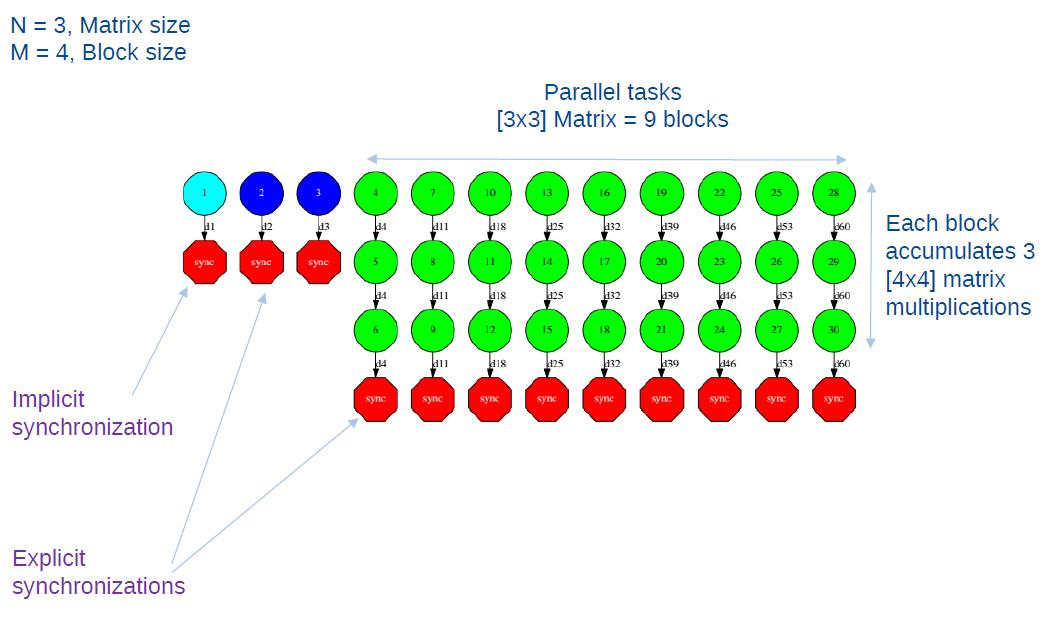
\includegraphics[width=1.0\textwidth]{./Sections/4_C/Figures/matmul.jpeg}
    \caption{Matmul Execution Graph.}
    %\label{fig:BLAST_workflow}
\end{figure}

  
  \section{Constraints}
\label{sec:Constraints}

This section provides a detailed information about all the supported constraints by the COMPSs runtime for 
\textbf{java}, \textbf{python} and \textbf{C/C++} languages. The constraints are defined as key-value pairs,
where the key is the name of the constraint. Table \ref{tab:constraints} details the available constraints names 
for \textit{Java}, \textit{Python} and \textit{C/C++}, its value type, its default value and a brief description.

\newpage

\begin{landscape}
\bgroup
  \def\arraystretch{1.3}%
  \begin{table}[]
  \centering
  \begin{tabular}{ | c | c | c | c | p{0.28\linewidth} | }
  \hline
  \textbf{Java} 		& \textbf{Python / C / C++}	& \textbf{Value type}	& \textbf{Default value}& \textbf{Description} \\ \hline
  computingUnits 		& ComputingUnits 		& $<$string$>$ 		& \"{}1\" 		& Required number of computing units \\ \hline
  processorName 		& ProcessorName 		& $<$string$>$ 		& \"{}[unassigned]\" 	& Required processor name \\ \hline
  processorSpeed 		& ProcessorSpeed 		& $<$string$>$ 		& \"{}[unassigned]\" 	& Required processor speed \\ \hline
  processorArchitecture 	& ProcessorArchitecture 	& $<$string$>$ 		& \"{}[unassigned]\" 	& Required processor architecture \\ \hline
  processorType			& ProcessorType		 	& $<$string$>$ 		& \"{}[unassigned]\" 	& Required processor type \\ \hline
  processorPropertyName		& ProcessorPropertyName 	& $<$string$>$ 		& \"{}[unassigned]\" 	& Required processor property \\ \hline
  processorPropertyValue	& ProcessorPropertyValue 	& $<$string$>$ 		& \"{}[unassigned]\" 	& Required processor property value \\ \hline
  processorInternalMemorySize 	& ProcessorInternalMemorySize 	& $<$string$>$ 		& \"{}[unassigned]\" 	& Required internal device memory \\ \hline
  processors 			& - 				& List$<$@Processor$>$  & \"{}\{\}\" 		& Required processors (check table \ref{tab:processor_constraint} for Processor details) \\ \hline
  memorySize	 		& MemorySize 			& $<$string$>$ 		& \"{}[unassigned]\" 	& Required memory size in GBs \\ \hline
  memoryType	 		& MemoryType 			& $<$string$>$ 		& \"{}[unassigned]\" 	& Required memory type (SRAM, DRAM, etc.) \\ \hline
  storageSize	 		& StorageSize 			& $<$string$>$ 		& \"{}[unassigned]\" 	& Required storage size in GBs \\ \hline
  storageType	 		& StorageType 			& $<$string$>$ 		& \"{}[unassigned]\" 	& Required storage type (HDD, SSD, etc.)\\ \hline
  operatingSystemType 		& OperatingSystemType 		& $<$string$>$ 		& \"{}[unassigned]\" 	& Required operating system type (Windows, MacOS, Linux, etc.)\\ \hline
  operatingSystemDistribution 	& OperatingSystemDistribution 	& $<$string$>$ 		& \"{}[unassigned]\" 	& Required operating system distribution (XP, Sierra, openSUSE, etc.)\\ \hline
  operatingSystemVersion 	& OperatingSystemVersion 	& $<$string$>$ 		& \"{}[unassigned]\" 	& Required operating system version \\ \hline
  wallClockLimit 		& WallClockLimit 		& $<$string$>$ 		& \"{}[unassigned]\" 	& Maximum wall clock time \\ \hline
  \cellcolor{blue!25} hostQueues  & HostQueues 			& $<$string$>$ 		& \"{}[unassigned]\" 	& Required queues \\ \hline
  \cellcolor{blue!25} appSoftware & AppSoftware 		& $<$string$>$ 		& \"{}[unassigned]\" 	& Required applications that must be available within the remote node for the task \\ \hline
  \end{tabular}
  \caption{Arguments of the \textit{@constraint} decorator}
  \label{tab:constraints}
  \end{table}
\egroup
\end{landscape}


All constraints are defined with a simple value except the {\it HostQueue} and {\it AppSoftware} constraints, which allow 
multiple values.

The \textit{processors} constraint allows the users to define multiple processors for a task execution. This constraint is specified
as a list of @Processor annotations that must be defined as shown in table \ref{tab:processor_constraint}

~ \newline

\bgroup
  \def\arraystretch{1.4}%
  \begin{table}[!ht]
  \centering
  \begin{tabular}{ | c | c | c | p{0.35\linewidth} | }
  \hline
  \textbf{Annotation} 	& \textbf{Value type}	& \textbf{Default value}& \textbf{Description} \\ \hline
  computingUnits 	& $<$string$>$ 		& \"{}1\" 		& Required number of computing units \\ \hline
  name 			& $<$string$>$ 		& \"{}[unassigned]\" 	& Required processor name \\ \hline
  speed 		& $<$string$>$ 		& \"{}[unassigned]\" 	& Required processor speed \\ \hline
  architecture 		& $<$string$>$ 		& \"{}[unassigned]\" 	& Required processor architecture \\ \hline
  type			& $<$string$>$ 		& \"{}[unassigned]\" 	& Required processor type \\ \hline
  propertyName		& $<$string$>$ 		& \"{}[unassigned]\" 	& Required processor property \\ \hline
  propertyValue		& $<$string$>$ 		& \"{}[unassigned]\" 	& Required processor property value \\ \hline
  internalMemorySize 	& $<$string$>$ 		& \"{}[unassigned]\" 	& Required internal device memory \\ \hline
  \end{tabular}
  \caption{Arguments of the \textit{@Processor} decorator}
  \label{tab:processor_constraint}
  \end{table}
\egroup
  
  \section{Known Limitations}
\label{sec:Known_Limitations}

The current COMPSs version (1.3) has the following limitations: 
\begin{itemize}
 \item \textbf{Exceptions:} \newline The current COMPSs version is not able to catch exceptions raised from a task.
 
 \item \textbf{Java tasks:} \newline Java tasks \textbf{must} be declared as \textbf{public}. Despite the fact that tasks can be
 defined in the main class or in other ones, we recommend to define the tasks in a separated class from the main method to force
 its public declaration.
 
 \item \textbf{Java objects:} \newline Objects used by tasks must follow the \textit{java beans} model (implementing an empty 
 constructor and getters and setters for each attribute) or implement the \textit{serializable} interface. This is due to the 
 fact that objects will be transferred to remote machines to execute the tasks.
 
 \item \textbf{Services types:} \newline The current COMPSs version only supports SOAP based services that implement the WS 
 interoperability standard. REST services are not supported.
 
 \item \textbf{Use of file paths:} \newline The persistent workers implementation has a unique \textit{Working Directory} per 
 worker. That means that tasks should not use hardcoded file names to avoid file collisions and tasks misbehaviors. We recommend to
 use files declared as task parameters, or to manually create a sandbox inside each task execution and/or to generate temporary 
 random file names. 
 
 \item \textbf{Tracing:} \newline The current version of the COMPSs tracing system slows down the application execution. Users
 running huge applications may experience a non-negligible overhead when using this feature. 
 
 \item \textbf{Intermediate files}: \newline Some applications may generate intermediate files that are only used among tasks
 and are never needed inside the master's code. However, COMPSs will transfer back these files to the master node at the end of the 
 execution. Currently, the only way to avoid transferring these intermediate files is to manually erase them at the end of the
 master's code. Users must take into account that this only applies for files declared as task parameters and \textbf{not} for files
 created and/or erased inside a task. 
 
 \item \textbf{Workers cache}: \newline Persistent workers maintain a cache to avoid transferring files and objects repeatedly. 
 However, this cache is \textbf{not} working for INOUT parameters (only works for IN and OUT parameters). For most applications, 
 if users are willing to exploit this cache, we recommend to convert INOUT parameters in \textbf{two} separated parameters: one 
 declared as IN parameter and the other declared as OUT parameter.
 
\end{itemize}



  %%%%%%%%%%%%% END PAGE %%%%%%%%%%%%%%
  \newpage

  \vspace*{\fill} 
  \begin{center}
    \large { Please find more details on the COMPSs framework at }
    \huge{\url{http://compss.bsc.es}}
  \end{center}    
  \vspace*{\fill} 
           
\end{document}
